\documentclass[a4paper,twoside,11pt]{report}
\usepackage[italian]{babel}
\usepackage[utf8x]{inputenc}
%\usepackage[latin1]{inputenc}
\usepackage[T1]{fontenc}
%\usepackage[scaled]{helvet}
%\renewcommand\familydefault{\sfdefault}

%\renewcommand{\sfdefault}{cmr}
%helvetica
%\renewcommand{\sfdefault}{phv}
%courier
%\renewcommand{\sfdefault}{pcr}
\usepackage{listings}
\usepackage{color}
\usepackage{caption}
\usepackage{subcaption}
\usepackage{sidecap}
\usepackage{quoting}
\quotingsetup{font=small}
\usepackage{eurosym}
\usepackage{graphicx}
\usepackage{epsfig}
\usepackage{url}
\usepackage{comment}
\usepackage{amsmath}
\usepackage[dvipsnames]{xcolor}
%%https://en.wikibooks.org/wiki/LaTeX/Colors
\usepackage[colorlinks]{hyperref}
%\hypersetup{hidelinks}

\hypersetup{%
	,urlcolor=Cyan
	,citecolor=black
	,linkcolor=black
}

\lstdefinestyle{customc}{
	belowcaptionskip=1\baselineskip,
	breaklines=true,
	frame=L,
	%xleftmargin=\parindent,
	language=C++,
	showstringspaces=false,
	basicstyle=\footnotesize\ttfamily,
	keywordstyle=\bfseries\color{green!40!black},
	commentstyle=\itshape\color{purple!40!black},
	identifierstyle=\color{blue},
	stringstyle=\color{orange},
}

\lstdefinestyle{customasm}{
	belowcaptionskip=1\baselineskip,
	frame=L,
	%xleftmargin=\parindent,
	language=[x86masm]Assembler,
	basicstyle=\footnotesize\ttfamily,
	commentstyle=\itshape\color{purple!40!black},
}

\lstset{escapechar=@,style=customc}


%opening
\title{Programmazione di Sistemi Embedded\\ {\Large Jimmy Challenge Arduino Game}}
\author{
    Edoardo Rosa - Matr. 707922\\
    Federico Torsello - Matr. 702619}

                             % \ip that is commented out.

\begin{document}             % End of preamble and beginning of text.
\maketitle                   % Produces the title.
\begin{abstract}

In questa relazione si descriverà come è stato progettato il gioco interattivo \textbf{Jimmy Challenge}, descrivendo le scelte di progettuali e le fasi implementative.

Jimmy Challenge è stato realizzato utilizzando diversi componenti hardware/software, con l'obiettivo di sfruttare ed ottimizzare quanto più possibile la board Arduino in un'ottica IoT.

\begin{description}
	\item [Capitolo 1] In questo capitolo si introduce il progetto e l'interazione giocatore-sistema.
	\item [Capotolo 2]
	
	
\end{description}


\end{abstract}
 %Sommario
\chapter{Introduzione}
\textbf{Jimmy Challenge}\footnote{"\textit{jimmy}" in inglese vuol dire grimaldello, da questo il nome del gioco.} è un gioco interattivo che si ispira all'attività di \textit{lock-picking}: aprire un lucchetto o una serratura usando ad esempio un \textbf{grimaldello} per manipolare i pistoncini interni per simulare la presenza della chiave originale.

Per poter giocare è necessario alimentare l'\href{https://www.arduino.cc/en/Main/ArduinoBoardUno}{Arduino UNO\footnote{Arduino UNO - è una scheda elettronica di piccole dimensioni con un microcontrollore ATmega, utile per creare rapidamente prototipi e per scopi hobbistici, didattici e professionali. (\url{https://it.wikipedia.org/wiki/Arduino\_\%28hardware\%29})}} e attendere qualche secondo di setup.

Una volta che il settaggio è completo, l'utente può interagire con Arduino utilizzando diversi componenti hardware che mutano il loro comportamento in base al contesto.





\chapter{Progettazione di un sistema Embedded}
\section{Analisi dei requisiti}
\subsection{Requisiti funzionali}
Il sistema realizzato deve permettere ad uno o due giocatori di competere per sbloccare dei lucchetti. Ad ogni lucchetto sbloccato si supera il livello fino a quando i livelli non terminano e il gioco si dice finito. Durante il gioco sono presenti delle penalità e dei bonus.

\subsection{Requisiti non funzionali}
Le performance utili per la buona riuscita del progetto a cui non si può rinunciare riguardano la rilevazione della distanza e l'invio dei feedback locali/remoti.
Il tempo gioca un ruolo importante in questo progetto, quindi si devono evitare inutili ritardi nella rilevazione ed invio delle informazioni.

\section{Modeling}
Il sistema si suddivide in più parti:
\begin{itemize}
	\item parte fisica lato client/server
	\item parte software lato client/server
	\item networking lato client/server
\end{itemize}

\subsection{Modellazione della parte fisica - lato client}
Dal punto di vista fisico, si ha un Arduino UNO:
 \begin{itemize}
 	\item connesso ad una breadboard e a dei componenti hardware attraverso i sui pin digitali
 	\item connesso ad un PC mediante la porta USB (da cui riceve l'alimentazione a 5v). 
 \end{itemize}
 Ogni componente della breadboard ha un proprio impiego distinguendoli in \textbf{sensori} ed \textbf{attuatori} secondo la visione di \textit{sistema reattivo}.

	\begin{quote}
		\textbf{Reactive system}: è l’ambiente esterno che determina gli eventi che
		condizionano l’esecuzione del sistema
	\end{quote}
	
La connessione seriale via USB serve per inviare i dati campionati dall'Arduino verso il PC. A loro volta questi dati possono servire per creare una GUI locale (per esempio su terminale) o remota, su browser.

\subsection{Modellazione della parte logica - lato client}
Per realizzare il comportamento dinamico del progettare, nella parte software si è replicato il funzionamento di una macchina a stati finiti (\textit{FSM}) che esegue dei task.

	\begin{quote}
		\textbf{Macchine a stati finiti} (o \textbf{\textit{automi a stati finiti}}): sono il modello nel discreto più utilizzato per modellare sistemi embedded.
		
		Ogni FSM opera in una sequenza di passi (discreti) e la sua dinamica è caratterizzata da sequenze di eventi (discreti).
		
		Un evento discreto avviene ad un determinato istante e non ha durata.
	\end{quote}
	
	\begin{quote}
		\textbf{Decomposizione in task}: principio di progettazione importante, rende modulare il sistema in quanto:
		\begin{itemize}
			\item ogni modulo è rappresentato da un task (compito da eseguire)
			\item un task può essere decomposto in sotto-task in modo ricorsivo o un task complesso può essere definito come composizione di sotto-task più semplici
		\end{itemize}
	\end{quote}
	
Si è fatto uso della modellazione ad oggetti, modellando ogni task come una classe separata che estende da una classe base task. In ogni task viene fatto l'\textbf{\textit{inject} del comportamento} da avere ad ogni tick.

Il multi-tasking realizzato è cooperativo, tipo round-robin in quanto c'è parallelismo e le funzioni tick() sono chiamate sequenzialmente all'interno del loop dello sheduler.

\begin{itemize}	
	\item si è fatto uso della programmazione Object-Oriented per rendere la struttura del codice ingegneristica, lineare e scalabile;
	\item si sono utilizzate le lambda expression per fare l'\textit{inject} di codice da eseguire nei vari task.
\end{itemize}

Per quanto riguarda la connessione USB, per scelta progettuale tutti i dati inviati dall'Arduino al PC sono tutti formattati in \textbf{JSON}.

\subsection{Modellazione della parte fisica - lato server}
\subsection{Modellazione della parte logica - lato server}
\section{Design}
Il sistema che si suddivide in più aree:
\begin{enumerate}
	\item I/O locale attraverso Arduino UNO
	\item feedback remoto su browser
	\item input per invio dei dati seriali al server attraverso async task Python
	\item connessione USB da Arduino UNO verso il PC
	\item connessione del PC ad un server
	\item sito internet come GUI remota
	\item gestione del server remoto
\end{enumerate}

Le tecno

– processo finalizzato alla creazione degli artefatti tecnologici che
rappresentano il sistema
– rappresentano come il sistema fa quello che deve fare
\section{Analysis}


Potenzialità software di Arduino UNO sfruttate:



Potenzialità hardware di Arduino UNO sfruttate:
\begin{itemize}
	\item sono stati utilizzati tutti i 12 pin di I/O digitale;
	\item si è cercato di limitare l'utilizzo di \textbf{delay} per mantenere le prestazioni ottimali;
	\item in alcuni casi al posto dei \textit{delay} si è fatto ricorso a dei \textbf{custom timer} impiegando il metodo \textbf{millis()};
\end{itemize}
\chapter{Giocare a Jimmy Challenge}
\section{Giocare con la mano e con i sensi}
L'obiettivo del giocatore è trovare e quindi scassinare il lucchetto nel minor tempo possibile. Questo gioco è giocabile \textbf{online} (uno contro uno) che \textbf{offline}.

La posizione del lucchetto viene assegnata in modo random ad ogni nuovo livello e rimane fissa fino al suo superamento.

Per trovare la posizione attuale del lucchetto al giocatore basta muovere la mano orizzontalmente in direzione del sensore ad ultrasuoni. (La rilevazione del lucchetto è spiegata più avanti).

Durante le varie fasi di gioco l'utente ha la possibilità di rendersi conto dell'evoluzione del gioco ascoltando i suoni emessi dal buzzer o guardando i colori dei LED.

\subsection{Significato dei suoni e dei colori}
\begin{itemize}
	\item All'avvio del gioco
	\begin{itemize}
		\item i LED a 12 pin giallo e rosso fanno un carosello;
		\item il LED verde e il buzzer si comportano come quando il lucchetto non è stato trovato.
	\end{itemize}
\end{itemize}


\begin{itemize}
	\item Quando \textbf{non} si è trovato il lucchetto:
	\begin{itemize}
		\item il LED verde emette una luce pulsante;
		\item il LED RGB emette una luce continua di color blu chiaro;
		\item il buzzer suona due note in modo frenetico.
	\end{itemize}
\end{itemize}

\begin{itemize}
	\item Quando si è nell'area del lucchetto:
	\begin{itemize}
		\item il LED verde emette una luce fissa;
		\item il LED RGB continuerà ad emettere una luce continua blu chiaro, ma solo fino a quando non entrerà nello stato di scasso;
		\item il buzzer suona due note meno freneticamente.
	\end{itemize}
\end{itemize}

\subsection{Superare un livello}
Per superare il livello il ladro deve forzare il lucchetto.

Dal punto di vista del giocatore il lucchetto è un'area nello spazio posta davanti al sensore (in linea orizzontale).

Per forzare il lucchetto è sufficiente utilizzare una mano posta davanti al sensore ad ultrasuoni per un tempo delimitato, avviando lo stato di scasso. Se il tempo di scasso non viene rispettato o la mano viene rimossa troppo presto, il livello riparte senza salvare i progressi.

\begin{itemize}
	\item \textbf{Non} si supera il livello:
	\begin{itemize}
			\item Se la mano viene spostata dall'area del lucchetto troppo presto, per esempio non si è ancora nello stato di scasso
			\item Se si rimane troppo tempo nella fase di scasso (il lucchetto è stato "rotto").
	\end{itemize}
\end{itemize}

\begin{itemize}
	\item Si può superare il livello:
	\begin{itemize}
			\item Se la mano resta fissa nella posizione in cui si trova il lucchetto, rispettando il tempo nello \textbf{stato di scasso} e poi la si agita sempre nell'area del lucchtto ("aprendolo").
	\end{itemize}
\end{itemize}

\subsection{Stato di scasso}
Se si rispetta il tempo nello stato di scasso e quindi si apre il lucchetto, si supera il livello.

Per indicare lo stato di scasso si è utilizzato il LED RGB. 
\begin{itemize}
	\item Ogni colore ha un significato:
	\begin{itemize}
		\item blu scuro: si sta scassinando il lucchetto
		\item verde: il lucchetto è scassinato.
			\subitem NB: per passare al livello successivo si deve togliere la mano e riposizionarla nell'area del lucchetto [come se si infilasse la "\textit{chiave}"].
		\item arancio: attenzione, se non si toglie la mano ora si rischia di rompere il lucchetto
		\item giallo: pericolo di rottura ancora più elevato
		\item rosso: il lucchetto è stato rotto, quindi il livello deve essere ricominciato di nuovo.
	\end{itemize}
\end{itemize}

Task:
\begin{itemize}
	\item SonarTask
	\item ButtonTask
	\item BuzzerTask
	\item LedTask
	\item LedPwmTask
	\item LedRgbTask
\end{itemize}
\chapter{Task}

\begin{figure}[!ht]
	\centering
	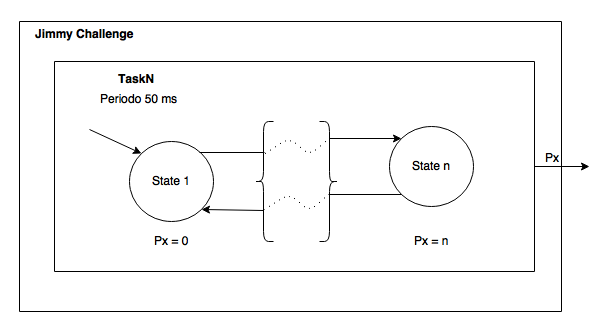
\includegraphics[scale=.60]{img/task_generic.png}
	\caption{Generalizzazione dei task}
\end{figure}

Task:
\begin{itemize}
	\item SonarTask
	\item ButtonTask
	\item BuzzerTask
	\item LedTask
	\item LedPwmTask
	\item LedRgbTask
\end{itemize}
\chapter{Classi concrete}
\section{Classi concrete sviluppate}
\begin{itemize}
	\item Classi utilizzate per l'\textbf{input}:
	\begin{enumerate}
		\item Sonar.cpp, Sonar.h;
		\item Button.cpp, Button.h.
	\end{enumerate}
	\item Classi utilizzate per l'\textbf{output}:
	\begin{enumerate}
		\item Buzzer.cpp, Buzzer.h;
		\item Led.cpp, Led.h;
		\item LedPwm.cpp, LedPwm.h;
		\item LedRgb.cpp, LedRgb.h;
		\item MessageService.cpp, MessageService.h;
		\item Multiplexer.cpp, Multiplexer.h.
	\end{enumerate}
	\item Classi utilizzate per coordinare il \textbf{multi-tasking}:
	\begin{enumerate}
		\item Context.h;
		\item Scheduler.cpp, Scheduler.h;
		\item Timer.h, Timer.cpp;
		\item Tash.h.
	\end{enumerate}
	\item Classi dei \textbf{task}:
	\begin{enumerate}
		\item ButtonTask.cpp, ButtonTask.h;
		\item BuzzerTask.cpp, BuzzerTask.h;
		\item LedPwmTask.cpp, LedPwmTask.h;
		\item LedRgbTask.cpp, LedRgbTask.h;
		\item LedTask.cpp, LedTask.h;
		\item SonarTask.cpp, SonarTask.h.
	\end{enumerate}
\end{itemize}

\section{Gestione dell'input}
\subsection{Sonar.cpp, Sonar.h}
Questa classe permette di leggere la distanza tra la mano del giocatore ed il sensore ad ultrasuoni.

Per ottenere un input molto performante dal punto di vista del tempo e dell'accuratezza, è stata sfruttata la libreria \href{http://playground.arduino.cc/Code/NewPing}{NewPing}.

In particolare nel costruttore di Sonar viene istanziato un oggetto \texttt{NewPing} a cui sono passati tre parametri:
\begin{itemize}
	\item \texttt{trigPin}: pin settato come output a cui è fisicamente collegato il trigger del sonar;
	\item \texttt{echoPin}: pin settato come output a cui è fisicamente collegato l'echo del sonar;
	\item \texttt{maxDistance}: limita massimo di distanza gestito oltre il quale la mano non viene rilevata e non si possono creare lucchetti.
\end{itemize}
\subsubsection{Metodi}
\begin{itemize}
	\item \texttt{int readDistance()}: lettura istantanea della distanza sensore-mano espressa in cm.
\end{itemize}
\begin{figure}[!ht]
	\centering
	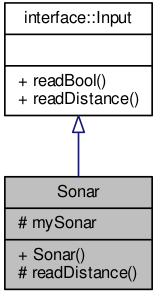
\includegraphics[scale=.5]{img/UML/CollaborationDiagram/Sonar.png}
	\caption{Collaboration Diagram - Sonar}
\end{figure}
\begin{figure}[!ht]
	\centering
	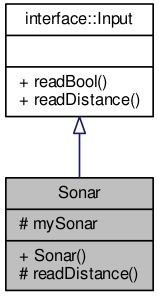
\includegraphics[scale=.5]{img/UML/InheritanceDiagram/Sonar.png}
	\caption{Inheritance Diagram - Sonar}
\end{figure}

\newpage
\subsection{Button.cpp, Button.h}
Anche questa classe implementa l'interfaccia Input. Lo scopo è riconoscere la pressione del button, evitando gli effetti del floating.

Il pin è stato configurato come \textit{INPUT\_PULLUP} in modo da sfruttare la resistenza interna dell'Arduino, ottenendo:
\begin{itemize}
	\item dei campionamenti con un rumori ridotti;
	\item floating del button quasi annullato.\footnote{Questa scelta di progetto è confermata dal tutorial: \href{http://tinyurl.com/jqp8nwu}{Arduino Internal Pull-Up Resistor}.}
\end{itemize}

\subsubsection{Metodi}
\begin{itemize}
	\item \texttt{bool readBool()}: prende come input il valore del pin disposto in configurazione INPUT\_PULLUP e lo nega. Se tale valore è falso viene campionato il tempo attuale. Se al successivo cambio di stato non è passato un tempo fissato e considerato sicuro, per evitare involontari cambi di stato, viene ignorato il segnale.
\end{itemize}
\begin{figure}[!ht]
	\centering
	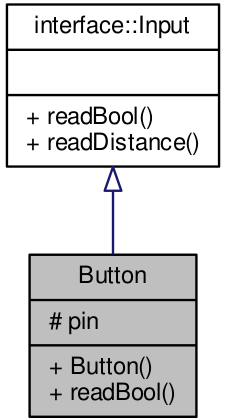
\includegraphics[scale=.35]{img/UML/CollaborationDiagram/Button.png}
	\caption{Collaboration Diagram - Button}
\end{figure}
\begin{figure}[!ht]
	\centering
	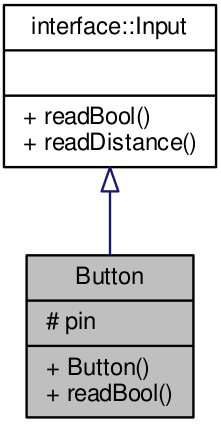
\includegraphics[scale=.35]{img/UML/InheritanceDiagram/Button.png}
	\caption{Inheritance Diagram - Button}
\end{figure}

\newpage
\section{Gestione dell'output}
\subsection{Buzzer.cpp, Buzzer.h}
Questa classe gestisce il buzzer, permettendo emettere dei suoni. Nel progetto è stato utile per far comprendere al giocatore lo stato di scasso del lucchetto.
\subsubsection{Metodi}
\begin{itemize}
	\item \texttt{public void playSound(const int sound)}: in base al numero intero passato a questo metodo, viene configurato il suono che il buzzer deve emettere;
	\item \texttt{private void playMarioTheme()}: un divertente easter egg;
	\item \texttt{private void buzz(int, int)}: modula le frequenze e le tonalità delle note che il buzzer deve emettere cambiando di stato da \texttt{HIGH} a \texttt{LOW} e viceversa.
\end{itemize}
\begin{figure}[!ht]
	\centering
	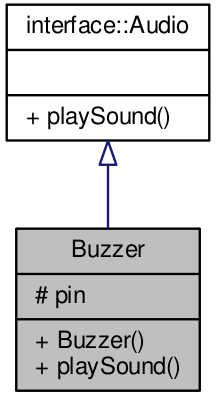
\includegraphics[scale=.35]{img/UML/CollaborationDiagram/Buzzer.png}
	\caption{Collaboration Diagram - Buzzer}
\end{figure}
\begin{figure}[!ht]
	\centering
	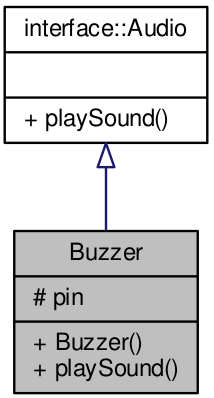
\includegraphics[scale=.35]{img/UML/InheritanceDiagram/Buzzer.png}
	\caption{Inheritance Diagram - Buzzer}
\end{figure}

\newpage
\subsection{Led.cpp, Led.h}
Classe per gestire l'accensione/spegnimento dei LED a 2 pin (controllo e massa) connessi all'Arduino.
\subsubsection{Metodi}
\begin{itemize}
	\item \texttt{protected	void switchOn()}: metodo che regola l'accensione istantanea del LED;
	\item \texttt{protected	void switchOff()}: metodo che regola lo spegnimento istantaneo del LED;
\end{itemize}
\begin{figure}[!ht]
	\centering
	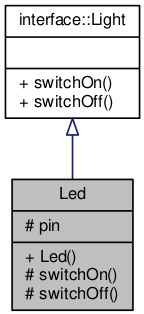
\includegraphics[scale=.5]{img/UML/CollaborationDiagram/Led.png}
	\caption{Collaboration Diagram - Led}
\end{figure}
\begin{figure}[!ht]
	\centering
	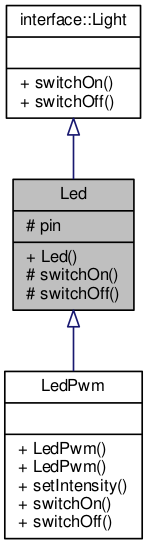
\includegraphics[scale=.5]{img/UML/InheritanceDiagram/Led.png}
	\caption{Inheritance Diagram - Led}
\end{figure}

\newpage
\subsection{LedPwm.cpp, LedPwm.h}
Questa classe permette l'accensione/spegnimento e dimmeraggio dei LED connessi ai pin PWM di Arduino
\subsubsection{Metodi}
\begin{itemize}
	\item \texttt{public void setIntensity(uint8\_t)}: imposta l'intensità luminosa emessa dal LED (compresa tra 0 e 255);
	\item \texttt{public void switchOn()}: imposta l'accensione istantanea del LED;
	\item \texttt{public void switchOff()}: imposta lo spegnimento istantaneo del LED;
\end{itemize}
\begin{figure}[!ht]
	\centering
	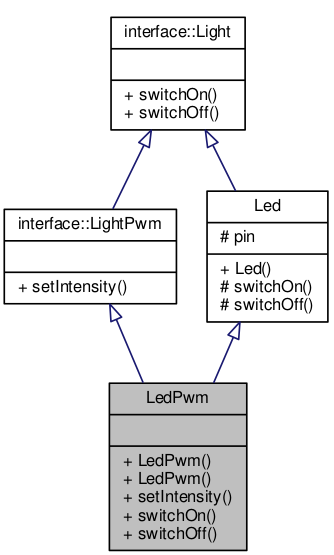
\includegraphics[scale=.4]{img/UML/CollaborationDiagram/LedPwm.png}
	\caption{Collaboration Diagram - LedPwm}
\end{figure}
\begin{figure}[!ht]
	\centering
	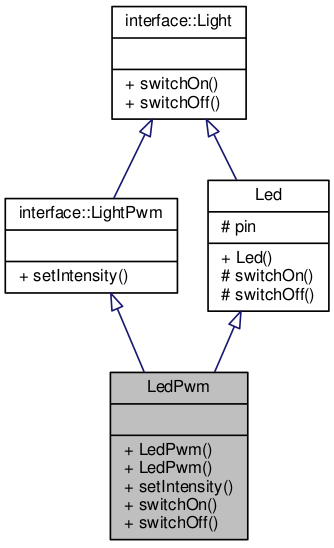
\includegraphics[scale=.4]{img/UML/InheritanceDiagram/LedPwm.png}
	\caption{Inheritance Diagram - LedPwm}
\end{figure}

\newpage
\subsection{LedRgb.cpp, LedRgb.h}
Questa classe permette il controllo dei LED RGB impostando i corretti pin per visualizzare il colore desiderato.

Nel dettaglio, il controllo viene eseguito istanziando tre oggetti \texttt{LedPwm} legati ad ogni colore/pin.
\subsubsection{Metodi}
\begin{itemize}
	\item \texttt{public void setColor(int, int, int)}: setta il colore da far vedere al giocatore;
	\item \texttt{protected	void switchOn()} : accensione istantanea del LED RGB;
	\item \texttt{protected	void switchOff()}: spegnimento istantaneo del LED RGB.
\end{itemize}
\begin{figure}[!ht]
	\centering
	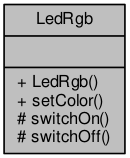
\includegraphics[scale=.5]{img/UML/CollaborationDiagram/LedRgb.png}
	\caption{Collaboration Diagram - LedRgb}
\end{figure}

\newpage
\subsection{Multiplexer.cpp, Multiplexer.h}
Classe che permette di gestire il multiplexer e quindi le sue uscite digitali. In questo progetto il multiplexer è strettamente legato ai LED a 12 pin regolando l'accensione/spegnimento di ogni LED interno. La classe è impostate per utilizzare la tabella di verità del multiplexer CD4067B.
\subsubsection{Metodi}
\begin{itemize}
	\item \texttt{public void switchOn(int)}: abilita il pin in uscita del multiplexer. Nel progetto è stato utile per visualizzare il livello a cui si sta giocando o il carosello sui LED a 12 pin;
	\item \texttt{public void carouselYellow(int)}: carosello del LED a 12 pin giallo, cioè si illuminano uno alla volta i LED interni per il periodo passato come intero;
	\item \texttt{public void carouselRed(int)}: carosello del LED a 12 pin rosso, con funzionamento identico al \texttt{carouselYellow(int)}.
\end{itemize}
\begin{figure}[!ht]
	\centering
	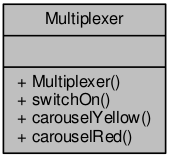
\includegraphics[scale=.5]{img/UML/CollaborationDiagram/Multiplexer.png}
	\caption{Collaboration Diagram - Multiplexer}
\end{figure}

\newpage
\subsection{MessageService.cpp, MessageService.h}
Questa classe permette di gestire l'invio e la ricezione di messaggi formattati in JSON attraverso la seriale.
Per codificare/decodificare i messaggi JSON è stata utilizzata la libreria \href{https://github.com/bblanchon/ArduinoJson}{ArduinoJson} (\ref{sec:arduinojason}), facilitando le operazioni di I/O su seriale.
\subsubsection{Metodi}
\begin{itemize}
	\item \texttt{public void init(const int, const String \&)}: inizializza la seriale e stampa un messaggio di inizalizzazione;
	\item \texttt{public void setMessage(String)}  quando un messaggio viene letto, è parsato, se valido viene inviato un \textit{ACK};
	\item \texttt{public void errorMsg()}: invia un messaggio di errore;
	\item \texttt{public void ackMsg(const String)} : invio di un \textit{ACK};
	\item \texttt{public void sendMsg(const String, const String)}: invia un messaggio al destinatario.
	\item \texttt{public void sendInfo(const int, const int, const uint8\_t, const String)}: invia un messagio di servizio utile all'aggiornamento dello stato della partita.
\end{itemize}
\begin{figure}[!ht]
	\centering
	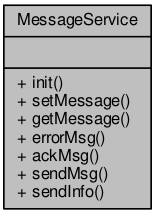
\includegraphics[scale=.5]{img/UML/CollaborationDiagram/MessageService.png}
	\caption{Collaboration Diagram - MessageService}
\end{figure}

\newpage
\section{Coordinamento dei task}
\section{Scheduler}
Lo Scheduler coordina l'esecuzione dei task secondo una schedulazione round-robin.

Al suo interno è presente un array \texttt{taskList} che contiene tutti i task da eseguire (aggiunti tramite \texttt{bool addTask(Task* task)}.

Nel caso in cui non ci siano task da eseguire o fossero tutti disabilitati, il sistema rimarrebbe apparentemente fermo (anche se in realtà il microcontrollore continuerebbe ad eseguire il suo \texttt{void loop()}).

Lo Scheduler è \textbf{cooperativo} in quanto una volta selezionato un task, questo viene eseguito fino al suo completamento (\textit{run-to-completion}).

Lo scheduling è a \textbf{priorità statica}, in quanto ad ogni task viene assegnata una priorità che non cambia durante l'esecuzione. La si può considerare come definita implicitamente dall'ordine di inserimento dei task nella \textit{task list}.

\subsection{Scheduler.cpp, Scheduler.h}
\subsubsection{Metodi}
\begin{itemize}
	\item \texttt{public void init(int)}: inizializza il base period dello Scheduler;
	\item \texttt{public virtual bool addTask(Task *)}: aggiunge il task alla lista dei task da eseguire;
	\item \texttt{public virtual void schedule()}: pianifica l'esecuzione dei vari task, eseguendoli uno alla volta. Nel caso in cui un task non sia abilitato, viene semplicemente ignorato (non eseguendo il suo tick) e quindi si passa immediatamente al successivo della lista.
\end{itemize}
\begin{figure}[!ht]
	\centering
	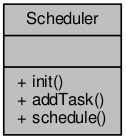
\includegraphics[scale=.5]{img/UML/CollaborationDiagram/Scheduler.png}
	\caption{Collaboration Diagram - Scheduler}
\end{figure}

\section{Context}\label{sec:contextimpl}
La classe Context contiene tutti le variabili di stato del programma. I metodi al suo interno sono accessibili da tutti i task in modo da far evolvere il sistema; di seguito la lista di tutti i metodi e del loro significato.
\subsection{Context.h}
\subsubsection{Metodi}
\begin{itemize}
	\item \texttt{bool isPadlockOpen(}): serve a sapere se il giocatore ha aperto il lucchetto;
	\item \texttt{void setPadlockOpen(bool padlockOpen)}: setting dello stato del lucchetto aperto/chiuso;
	\item \texttt{bool isPadlockDetected()}: serve a sapere se il giocatore ha trovato la giusta posizione del pistoncino;
	\item \texttt{void setPadlockDetected(bool padlockDetected)}: set dello stato del pistoncino trovato o no;
	\item \texttt{void setCurrentDistance(int currentDistance)}: set della distanza del padlock da aprire;
	\item \texttt{int getCurrentDistance()}: restituisce la distanza a cui si trova la mano;
	\item \texttt{void setButtonPressed(bool buttonPressed)}: set dello stato del bottone, se premuto o no;
	\item \texttt{bool isButtonPressed()}: restituisce lo stato del bottone;
	\item \texttt{void setNewLevel()}: crea il nuovo livello da giocare;
	\item \texttt{uint8\_t getDelta()}: margine di errore della posizione del pistoncino;
	\item \texttt{uint8\_t getLevel()}: restituisce il livello attuale;
	\item \texttt{int getSecret()}: restituisce la distanza a cui si trova il lucchetto;
	\item \texttt{void newRandomNumber(}): genera un nuovo numero random;
	\item \texttt{void setGameOver(bool gameOver)}: setta lo stato del gioco, cioè se è finito o no;
	\item \texttt{bool isGameOver()}: restituisce lo stato del gioco, finito o no;
	\item \texttt{void setDangerLevel (uint8\_t dangerLevel)}:  set del livello di pericolo nello stato di scasso;
	\item \texttt{uint8\_t getDangerLevel()}: restituisce il livello di pericolo nello stato di scasso;
	\item \texttt{void setLockpicking (bool state)}: set dello stato di scasso;
	\item \texttt{bool isLockpicking()}: indica se ci si trova nello stato di scasso;
	\item \texttt{void carousel(uint8\_t delay1, uint8\_t delay2)}: esegue un carosello temporizzato dei due LED a 12 pin.
\end{itemize}
\begin{figure}[!ht]
	\centering
	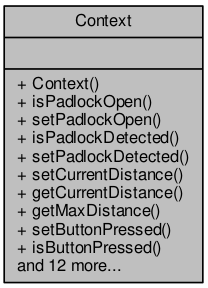
\includegraphics[scale=.5]{img/UML/CollaborationDiagram/Context.png}
	\caption{Collaboration Diagram - Context}
\end{figure}

\subsection{Timer.h, Timer.cpp}
\subsubsection{Metodi}
\begin{itemize}
	\item public void setupPeriod(int): disabilita gli \textit{interrupt}, setta i registri del Timer1 (configurando il prescale) e riabilita gli interrupt;
	\item public void waitForNextTick(): permette di eseguire il task.
\end{itemize}
\begin{figure}[!ht]
	\centering
	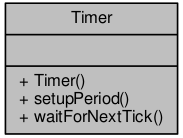
\includegraphics[scale=.5]{img/UML/CollaborationDiagram/Timer.png}
	\caption{Collaboration Diagram - Timer}
\end{figure}

\chapter{Multi-Tasking}

\section{Task}
I task rappresentano le azioni da eseguite concorrentemente nel sistema, pianificate dallo Scheduler. 

\begin{itemize}
	\item Dal \textbf{punto di vista del progettista}:
	\begin{itemize}
		\item sono delle entità attive dotate di un flusso di controllo autonomo che svolgono un determinato compito e che impegnano il microprocessore per un certo periodo;
		\item permettono di elaborare dati provenienti dai sensori ed agire sugli attuatori e/o gestire eventi I/O;
		\item possono essere sostituiti, alterati, inibiti o modificati in base alle necessità.
	\end{itemize}
	\item Dal \textbf{punto di vista dell'utente} invece:
	\begin{itemize}
		\item  creano l'illusione di avere un unico sistema monolitico;
		\item  la semplice esistenza e quindi la loro gestione è trasparente all'utente.
	\end{itemize}
\end{itemize}
Per la descrizione del comportamento di ogni task, si è deciso di utilizzare le lambda expression (\ref{sec:lambda}). 

In sintesi i vari task sono istanziati definendo all'interno del \textit{body} del metodo \texttt{init(...)} ogni singolo \textit{behaviour}. Per farlo sono utilizzati: 
\begin{itemize}
	\item i metodi propri del task;
	\item i metodi del Context \ref{sec:context} come mezzo di comunicazione tra i diversi task.
\end{itemize}
Questo ci ha permesso di avere più gradi di libertà nella definizione del comportamento dei task e quindi del codice da eseguire. In quest'ottica non vi è necessità di creare una classe per ogni singolo comportamento, ma basta istanziare due o più volte la classe e definire diversi body.

\subsubsection{Esempio}
Si vogliono controllare due LED utilizzando il task LedTask; in particolare:
\begin{itemize}
	\item se viene trovato il lucchetto, il led1 viene acceso e il led2 viene spento,
	\item altrimenti, se il lucchetto non viene trovato, il led1 passa a spento e il led2 diventa acceso.
\end{itemize}
\begin{lstlisting}[language=C++,frame=none]
ledT0 = new LedTask(led1, pContext);
ledT0->init(50, [] {
   	if (pContext->isPadlockDetected()) {
   	  ledT0->led->switchOn();
   	} else {
   	  ledT0->led->switchOff();
	}
});
sched.addTask(ledT0);

ledT1 = new LedTask(led2, pContext);
ledT1->init(50, [] {
   	if (pContext->isPadlockDetected()) {
	  ledT1->led->switchOn();
   	} else {
   	  ledT1->led->switchOff();
	}
});
sched.addTask(ledT1);
\end{lstlisting}
Dopo la creazione, il task per eseguire deve essere aggiunto alla lista di esecuzione dello Scheduler; per farlo si usa \texttt{sched.addTask(<nome del task>)}.

\subsection{Le espressioni Lambda in Wiring/C++11}\label{sec:lambda}
Una \textbf{Lambda expression} (\textit{lambda closure}) è una funzione anonima definita al momento della chiamata. 

Sintassi accettate dal compilatore di Arduino:
\begin{lstlisting}[language=C++,frame=none]
[ capture-list ] ( params ) { body }
[ capture-list ] { body } 
\end{lstlisting}

\subsubsection{Caratteristiche}
\begin{itemize}
	\item La \textit{capture list} è la lista di variabili che è possibile utilizzare oltre agli argomenti della funzione.
	\begin{itemize}
		\item Se si passa \texttt{[\&]}, tutte le variabili locali saranno passate per riferimento.
		\item Se non viene specificato niente, la \textit{lambda function} non ha variabili come argomenti e viene indicata con \texttt{[]};
	\end{itemize}
	\item Il tipo di ritorno è \texttt{void}, a meno che non venga specificato diversamente;
	\item Il body della funzione che si trova tra parentesi graffe.
\end{itemize}

\subsubsection{Vantaggi}
\begin{itemize}
	\item è possibile creare una classe "generica" che può avere più istanze a cui assegnare più behaviour;
	\item si evita di dover creare per ogni comportamento una classe specifica;
	\item codice modulare, (diverse istanze dello stesso oggetto possono avere diversi body);
	\item definizione del comportamento direttamente dal file \texttt{*.ino}.
\end{itemize}

\subsubsection{Contro}
Per utilizzare le lambda expression siamo stati costretti a rinunciare parzialmente all'\textit{information hiding} della programmazione OO. Questo vincolo è legato al fatto che non è stato possibile passare oggetti come parametro di chiusura a causa di alcuni vincoli del linguaggio usato da Arduino.

L'unico modo per passare gli oggetti e quindi i metodi all'interno di queste particolari funzioni è stato mettere tutto \texttt{public}.

\subsection{Generalizzazione del funzionamento di un task}
\begin{figure}[!ht]
	\centering
	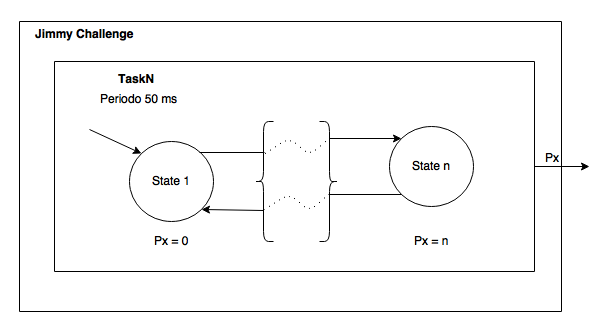
\includegraphics[scale=.60]{img/task_generic.png}
	\caption{Generalizzazione dei task}
\end{figure}

\subsubsection{Elenco dei Task sviluppati:}
\begin{enumerate}
	\item SonarTask
	\item ButtonTask
	\item BuzzerTask
	\item LedTask
	\item LedPwmTask
	\item LedRgbTask
\end{enumerate}

\subsection{SonarTask}
È il task più importante del progetto in quanto:
\begin{itemize}
	\item permette l'interazione utente-sistema sfruttando il sensore ad ultrasuoni;
	\item aggiorna la \texttt{currentDistance} del Context (\ref{sec:context});
	\item in modo indiretto può variare l'evoluzione del sistema
\end{itemize}
Nella classe SonarTask viene definito il metodo \texttt{private playLevel()} in cui:
\begin{itemize}
	\item si legge la currentDistance dal sonar;
	\item si setta tale currentDistance nel Context;
	\item si gestiscono gli \texttt{status} da inviare alla seriale
\end{itemize}

Dal Context:
\begin{itemize}
	\item si riceve il \textbf{numero segreto}: la distanza del pistoncino a partire dal punto 0, ovvero il sonar);
	\item si riceve il \textbf{delta}: intervallo di errore in cui la posizione del pistoncino è considerata corretta;
	\item si riceve il \textbf{livello attuale} a cui si sta giocando;
	\item si controlla se il lucchetto è aperto con \texttt{pContext->isPadLockOpen()}
\end{itemize}
Sul Context:
\begin{itemize}
	\item se il lucchetto è stato aperto si crea un nuovo livello con \texttt{pContext->setNewLevel()};
	\item se il padLock non è stato completamente sbloccato viene settato come chiuso con \texttt{pContext->setPadlockOpen(false)};
	\item se il padLock non è stato completamente sbloccato viene resettato lo stato di scasso con \texttt{pContext->setLockpicking(false)};
	\item in base al tempo passato nello scassinare il lucchetto (e quindi allo \texttt{status} in cui ci si trova), viene settato \texttt{pContex->setDangerLevel(...)} con un numero da 0 a 4, (che nel LedRgbTask indica il colore da visualizzare sul LED RGB).
\end{itemize}

\begin{lstlisting}[language=C++,frame=none]
void SonarTask::playLevel() {
	currentDistance = sonar->readDistance();
	pContext->setCurrentDistance(currentDistance);
	int secretDistance = pContext->getSecret();
	int currentLevel = pContext->getLevel();
	uint8_t delta = pContext->getDelta();
	int status = 0;
	int feedbackDistance = 0;
	
	feedbackDistance = abs(currentDistance - secretDistance);
	if (feedbackDistance == 0)
		feedbackDistance = 0;
	else if (currentDistance == 0)
		feedbackDistance = 100;
	
	if(currentDistance <= (secretDistance + delta)
	&& currentDistance >= (secretDistance - delta)) {
		pContext->setPadlockDetected(true);
		timeFound = (millis()/1000) - timeOut;     // inizializzazione a zero
		switch (timeFound) {
			case 0:
			if (pContext->isPadlockOpen()) {
				msgService.sendMsg("Lucchetto livello " + String(currentLevel) + " APERTO", F("all"));
				pContext->setNewLevel();
				if (!pContext->isGameOver()) {
					status = 300 + currentLevel + 1;
					pContext->setPadlockOpen(false);
					pContext->setLockpicking(false);
				}
			} else
			status = 101;
			break;
			case 1:
			status = 101;
			break;
			case 2:
			status = 102;
			break;
			case 3:
			status = 103;
			break;
			case 4:
			status = 104;
			pContext->setDangerLevel(0);
			pContext->setLockpicking(true);
			break;
			case 5:
			status = 104;
			pContext->setDangerLevel(0);
			break;
			case 6:
			status = 105;
			pContext->setDangerLevel(1);
			pContext->setPadlockOpen(true);
			break;
			case 7:
			status = 201;
			pContext->setDangerLevel(1);
			break;
			case 8:
			status = 202;
			pContext->setDangerLevel(2);
			break;
			case 9:
			status = 203;
			pContext->setDangerLevel(3);
			break;
			case 10:
			status = 204;
			pContext->setDangerLevel(4);
			pContext->setPadlockOpen(false);
			break;
			case 11:
			status = 205;
			pContext->setDangerLevel(4);
			break;
		}
	} else {
	timeOut = millis()/1000;
	pContext->setPadlockDetected(false);
	pContext->setLockpicking(false);
}
msgService.sendInfo(currentDistance, status, currentLevel, F("remote"));
}
\end{lstlisting}

Per la rilevazione della distanza della mano dal sensore è stata utilizzata la libreria \textbf{NewPing} \ref{sec:newping}.


\subsection{ButtonTask}
Questo task controlla se è avvenuta la pressione del \textit{button}.
Finché il gioco non è finito è possibile stampare su terminale un messaggio che indica la posizione del lucchetto. 

Se il gioco è finito, ma il bottone viene comunque premuto, si avvia una divertente \textbf{\textit{easter egg}} legata al BuzzerTask e ad un famoso gioco degli anni '80\dots


\subsection{BuzzerTask}
Questo task controlla i suoni che il \textit{buzzer} deve emettere attraverso il metodo \texttt{buzzerT0->buzzer->playSound(<num>)}

\begin{itemize}
	\item Se il gioco non è finito e il lucchetto non è ancora stato trovato, viene emesso il suono 0;
	\item Se il gioco non è finito e il lucchetto è stato trovato, viene emesso il suono 1;
	\item Se il gioco è finito e il pulsante premuto, viene emesso il suono 2 (\textbf{\textit{easter egg}}).
\end{itemize}

\subsection{LedTask}
Questo task controlla l'accensione e lo spegnimento del LED verde.

\begin{itemize}
	\item Se il gioco non è finito e il lucchetto è stato trovato, il LED viene acceso;
	\item Se il gioco non è finito e il lucchetto non è ancora stato trovato, il LED viene spento.
\end{itemize}

\subsection{LedPwmTask}
Questo task gestisce il LED verde utilizzando il pin PWM grazie ai seguenti metodi:
\begin{itemize}
	\item \texttt{ledPwmT0->ledPwm->setIntensity(<num>)} per gestire l'intensità luminosa (anche temporizzata) del LED;
	\item \texttt{ledPwmT0->ledPwm->switchOff()} per spegnere immediatamente il LED.
\end{itemize}
Analizzando questo task nel dettaglio:
\begin{itemize}
	\item Se il lucchetto non è stato aperto e non è stato trovato:
	\begin{itemize}
		\item si aumenta l'intensità del LED usando un ciclo \texttt{for} inizializzato a 64 (in modo da non partire dal LED completamente spento) per arrivare a 255 (valore massimo consentito).
		\item al termine del ciclo il LED viene spento
	\end{itemize}
	L'obiettivo di questo frammento di codice è far capire al giocatore che il sistema è in funzione facendo illuminare e subito spegnere il LED, come se questo emettesse tanti flash luminosi.
	\item Se il gioco è finito:
	\begin{itemize}
		\item si aumenta l'intensità del LED usando un ciclo \texttt{for} inizializzato a 10 (riducendo il tempo necessario per arrivare al massimo).
		\item all'interno di questo ciclo è stato inserito un \textbf{delay} di 3 ms per rendere più visibile il dimmeraggio
		\item al termine del ciclo for, il LED viene spento.
	\end{itemize}
\end{itemize}

\subsection{LedRgbTask}
Questo task gestisce il funzionamento del LED RGB.

In fase di creazione prende in input i pin PWM dell'Arduino a cui è collegato fisicamente il LED RGB (costanti \texttt{LED\_RGB\_R}, \texttt{LED\_RGB\_G}, \texttt{LED\_RGB\_B}).

Funzionamento:
\begin{itemize}
	\item Finché il gioco non è finito:
	\begin{itemize}
		\item Se si è in fase di scasso, si imposta un colore nel costrutto swhitch-case in base al numero intero di \texttt{pContext->getDangerLevel()}
			\item Nel dettaglio:
			\begin{itemize}
				\item 0 = \textbf{blu scuro} (inizio stato di scasso); 
				\item 1 = \textbf{verde} (lucchetto sbloccato);
				\item 2 = \textbf{giallo} (attenzione, rischio di rompere il lucchetto);
				\item 3 = \textbf{rosa} (attenzione, elevato pericolo di rottura);
				\item 4 = \textbf{rosso} (rottura del lucchetto).
			\end{itemize}
		\item Altrimenti si imposta un colore \textbf{\textit{light blue}} costante.
	\end{itemize}
\end{itemize}

\section{Scheduler}
Lo Scheduler coordina e fa cooperare i task del sistema.

Al suo interno è presente il vettore \texttt{taskList[...]} in cui sono aggiunti i task da eseguire grazie al metodo \texttt{bool addTask(Task* task)}.

Nel caso in cui nello Scheduler non ci fossero task o fossero stati tutti bloccati, il sistema rimarrebbe apparentemente fermo (anche se in realtà il microcontrollore continuerebbe ad eseguire il suo \texttt{void loop()}).

Lo Scheduler è \textbf{cooperativo} in quanto una volta selezionato un task, questo viene eseguito fino al suo completamento (\textit{run-to-completion}). Ad ogni tick della FSM vengono eseguite atomicamente le azioni associate al nuovo stato.

Lo scheduling è a \textbf{priorità statica}, in quanto ad ogni task viene assegnata una priorità che non cambia durante l'esecuzione. La si può considerare come definita implicitamente dall'ordine di inserimento dei task nella \textit{task list}.

\section{Context}\label{sec:context}
La classe Context contiene tutti le variabili di stato del programma. I metodi al suo interno sono accessibili da tutti i task in modo da far evolvere il sistema; di seguito la lista di tutti i metodi e del loro significato.

\subsubsection{Metodi}
\begin{itemize}
	\item \texttt{bool isPadlockOpen(}) : serve a sapere se il giocatore ha aperto il lucchetto;
	\item \texttt{void setPadlockOpen(bool padlockOpen)} : setting dello stato del lucchetto aperto/chiuso;
	\item \texttt{bool isPadlockDetected()} : serve a sapere se il giocatore ha trovato il lucchetto, cioè la distanza giusta dal sensore;
	\item \texttt{void setPadlockDetected(bool padlockDetected)} : set dello stato del padlock trovato o no;
	\item \texttt{void setCurrentDistance(int currentDistance)} : set della distanza del padlock da aprire;
	\item \texttt{int getCurrentDistance()} : restituisce la distanza a cui si trova la mano;
	\item \texttt{void setButtonPressed(bool buttonPressed)} : set dello stato del bottone, se premuto o no;
	\item \texttt{ bool isButtonPressed()} : restituisce lo stato del bottone;
	\item \texttt{void setNewLevel()} : crea il nuovo livello da giocare;
	\item \texttt{uint8\_t getDelta()} : margine di errore come scarto;
	\item \texttt{uint8\_t getLevel()} : restituisce il livello a cui si sta giocando;
	\item \texttt{int getSecret()} : restituisce la distanza a cui si trova il lucchetto;
	\item \texttt{void newRandomNumber(}) : genera un nuovo numero random;
	\item \texttt{void setGameOver(bool gameOver)} : setta lo stato del gioco, cioè se è finito o no;
	\item \texttt{bool isGameOver()} : restituisce lo stato del gioco, finito o no;
	\item \texttt{void setDangerLevel (uint8\_t dangerLevel)} :  set del livello di pericolo nello stato di scasso;
	\item \texttt{uint8\_t getDangerLevel()} : restituisce il livello di pericolo nello stato di scasso;
	\item \texttt{void setLockpicking (bool state)} : set dello stato di scasso;
	\item \texttt{bool isLockpicking()} : indica se ci si trova nello stato di scasso;
	\item \texttt{void carousel(uint8\_t delay1, uint8\_t delay2)} : esegue un carosello temporizzato dei due LED a 12 pin.
\end{itemize}




\section{Networking e Sicurezza}

Il mondo embedded e IoT in questi anni sta avendo un forte sviluppo, grazie alla disponibilità di dispositivi dal rapporto prestazioni/prezzo vantaggioso, e ha creato un grande bacino di utenza di esperti, o semplici neofiti, interessati al mondo dell'elettronica/informatica dedicata. Un effetto positivo di questa evoluzione è lo sviluppo di librerie open-source e di sistemi software orientati all'IoT.

Questo trend ha creato un mercato sempre più vasto di produttori di dispositivi più performanti, economici e dalle dimensioni ridotte (perfetti per realizzazioni embedded).
A causa di questo sviluppo, per certi versi incontrollato, "tutto" è virtualmente collegato/collegabile \textit{online} e sembra essere passata in secondo piano la progettazione di hardware e software che tiene conto della \textbf{sicurezza dei sistemi}. I primi attacchi mirati a queste tecnologie hanno avuto facilità di esecuzione e una rapidissima diffusione\footnote{Breve lista di attacchi a sistemi IoT nel 2015 \url{http://tinyurl.com/honlko2}.}.

In questo scenario, dalla parte dei produttori hardware si registra una mancanza o addirittura una resistenza per quanto riguarda la correzione di falle o il rilascio di aggiornamenti firmware. Questo potrebbe essere dovuto all'utilizzo di codice proprietario o la totale mancanza di supporto per il dispositivo che si utilizza. In alcuni casi si potrebbe parlare di \textbf{obsolescenza programmata}.

Anche da parte degli utilizzatori finali dei sistemi non si evince una particolare attenzione ai problemi relativi alla sicurezza; probabilmente a causa delle scarse conoscenze del sistema in uso (perché complesso o non studiato) e delle tecnologie usate. È ormai tristemente noto che lo sviluppo di questi \textbf{\textit{dispositivi perennemente connessi}}, non prende quasi mai in considerazione le problematiche relative alla sicurezza derivata dalla connessione a sistemi più \textit{fragili} o legate all'interazione con altri device (perdita di privacy, prestazioni o utilizzo improprio di risorse di rete).\\

Jimmy Challenge è stato sviluppato garantendo la sicurezza del sistema e dei giocatori.\\

In questo capitolo verranno presentate alcune delle soluzioni adottate e delle tecnologie utilizzate per l'implementazione dell'applicativo lato server e dei collegamenti di reti.
Per scelta progettuale ed etica, ove possibile, si è preferito utilizzare esclusivamente software \textit{open-source}.

\subsection{Sistema Operativo}
Le mansioni di server sono fisicamente compiute da un \textbf{Odroid C2}) il quale utilizza come OS una versione ARM a 64-bit della distribuzione Linux \textbf{Arch Linux ARM}.

\subsubsection{Arch Linux ARM} 
\begin{itemize}
	\item è \textit{bleeding edge} per quanto riguarda l'upstream degli aggiornamenti (sempre aggiornata all'ultima versione dei software disponibile);
	\item generalmente è considerata sicura;
	\item fornisce una libertà maggiore per la configurazione del sistema;
	\item una forte e grande community.
\end{itemize}

\subsubsection{Software installato orientato alla sicurezza}
\begin{itemize}
	\item \textbf{SSH} con autenticazione chiave pubblica-privata RSA;
	\item firewall \textbf{UFW}, per rendere disponibili all'esterno soltanto alcuni servizi;
	\begin{itemize}
		\item 80: Web Server;
		\item 22: SSH;
		\item 443: HTTPS.
	\end{itemize}
	\item \href{https://certbot.eff.org/}{Cerbot} per i certificati SSL/TLS;
	\item\href{https://github.com/firehol/netdata}{Netdata}  per una visualizzazione delle risorse del sistema da remoto.
\end{itemize}
Oltre all'installazione e alla configurazione dei software sono stati configurati diversi parametri per l'\textit{hardening} del kernel tramite \textit{sysctl} ed un sistema di \textit{logging} per la registrazione degli accessi.

\subsection{NGINX e HTTPS}
\textbf{NGINX} è un web server orientato alle performance, al ridotto consumo di risorse e alla facilità di configurazione.
In un sistema come l'Odroid con potenza computazionale ridotta (rispetto ai classici server) l'utilizzo di applicativi con ridotto consumo di risorse garantisce una maggiore reattività del sistema e un migliore risultato agli occhi dell'utente.

La configurazione di NGINX prende in considerazione tutti i maggiori problemi legati all'esposizione di un sito e di un web server in rete: buffer overflow, DDoS, bruteforcing, sniffing, etc. e cerca di mitigare o prevenire ogni tipo di attacco senza generare intralcio o rallentamenti all'utilizzo standard del web server.\\
Grazie a \textit{Cerbot} è possibile ottenere certificati SSL/TLS gratuitamente e garantire un canale di comunicazione protetto tra client e server.\\
La configurazione di NGINX è visibile \href{https://raw.githubusercontent.com/FedericoTorsello/Embedded/serverPHP/nginx.conf}{qui}.\\
L'intera configurazione di NGINX cerca di essere compatibile con gli ultimi protocolli e limitare quelli obsoleti e poco sicuri, rischiando però di ridurre la compatibilità con i browser minori. Per garantire ulteriori performance NGINX è abilitato ad instaurare connessioni tramite il recente protocollo HTTP/2 con i client compatibili.

\subsection{MySQL, Redis}
MySQL e Redis:
\begin{itemize}
	\item non sono esposti verso l'esterno;
	\item sono protetti da password;
	\item sono configurati per rispettare il POLP (\textit{principle of least privilege}).
\end{itemize}
\subsubsection{MySQL}
Con \textbf{MySQL} si gestisce il database per lo storage delle credenziali degli utenti e la lista degli utenti connessi online.
\begin{lstlisting}[frame=none]
CREATE TABLE IF NOT EXISTS users (
id int(3) NOT NULL AUTO_INCREMENT PRIMARY KEY,
created DATETIME DEFAULT CURRENT_TIMESTAMP,
username varchar(15) COLLATE utf8_general_ci NOT NULL,
password varchar(255) COLLATE utf8_general_ci NOT NULL,
email varchar(30) COLLATE utf8_general_ci NOT NULL,
keepalive DATETIME DEFAULT CURRENT_TIMESTAMP ON UPDATE CURRENT_TIMESTAMP,
logged boolean NOT NULL DEFAULT 0,
) ENGINE=InnoDB DEFAULT CHARSET=utf8 COLLATE=utf8_general_ci;

ALTER TABLE users ADD INDEX logged_index(logged);

SET GLOBAL event_scheduler = ON;

DELIMITER $$
CREATE EVENT IF NOT EXISTS `keepalive_logged`
ON SCHEDULE EVERY 1 MINUTE STARTS '2016-06-01 00:00:00'
ON COMPLETION PRESERVE
DO BEGIN
UPDATE users SET logged = 0
WHERE TIMESTAMPDIFF(SECOND, keepalive, now()) >= 20;
END;$$
DELIMITER ;
\end{lstlisting}
Un event MySQL controlla periodicamente se un utente è ancora collegato o meno.

\subsubsection{Redis}
\textbf{Redis} è un applicativo per lo store di strutture dati chiave-valore in memoria. Il principale vantaggio di Redis è la sua velocità in lettura e scrittura e la facilità di utilizzo.

\subsection{Sito Web, back-end e API RESTful}
Il sito web (sia front-end che back-end) è stato sviluppato tenendo a mente le linee guida del W3C e del OWASP.

Al fine di rendere l'applicativo il più possibile portabile, sono state implementate delle API RESTful in PHP7; sia l'applicativo Python lato client, sia il sito web (tramite AJAX) utilizzano queste API.

Una volta che un utente si è loggato, gli viene assegnato un \textit{token} JWS (JSON Web Signature) che deve essere validato ad ogni richiesta che farà da quel momento in poi. Questo token permette di verificare l'identità dell'utente ad ogni richiesta ed evitare usi improri della API da utenti malintenzionati.
Le API possono essere invocate solo tramite richieste POST e comunicano tramite messaggi JSON appositamente formattati.

In seguito al login effettuato, il sito web si presenta all'utente come un'unica pagina in cui è possibile inviare messaggi a tutti gli altri utenti collegati tramite una chat globale e selezionare un giocatore da sfidare. 

Una volta iniziata una partita, nella view principale della pagina appariranno i dati relativi allo stato della partita dell'avversario. Ogni aggiornamento dello stato verso i client è effettuato tramite Server-Sent Events (SSE).

Grazie a SSE, per mezzo del pattern \textbf{publish-subscribe}:
\begin{itemize}
	\item si riducono i consumi di risorse computazionali
	\item si limita l'utilizzo della banda
	\item si eliminano i problemi di gestione di altre tecnologie come WebSocket o WebRTC.
\end{itemize} 
Per farlo si instaura un canale mono direzionale verso il client in cui è possibile istruire il browser per controllare periodicamente l'aggioranemto dello stato dei dati o forzare l'invio di dati aggioranti da parte del server.

Per il back-end sono state utilizzate diverse librerie per fornire alcune funzionalità come JWS e SSE scelte appositamente per la loro compatibilità con gli ultimi standard e versioni di PHP al fine di garantire maggiori performance e sicurezza:
\begin{itemize}
	\item \href{https://github.com/namshi/jose}{jose}: per i token JWS;
	\item \href{https://github.com/licson0729/libSSE-php}{libSSE-php}: per SSE;
	\item \href{https://github.com/symfony/http-foundation}{http-foundation} e \href{https://github.com/nrk/predis}{predis}: come dipendenze di "libSSE-php".
\end{itemize}
Le interazioni tramite il database MySQL avvengono per mezzo di una connessione locale, utilizzando le varie tecniche di mitigazione per SQLi di primo e secondo livello fornite dal PHP.

Per proteggere la privacy degli utenti, le password sono salvate sul database come hash (usando bcrypt).

\subsection{Python}
Come anticipato nella relazione, per poter inviare al server i dati letti dalla seriale di Arduino è stato sviluppato uno script Python, in particolare \textbf{Python 3.5}.

\begin{figure}[!ht]
	\centering
	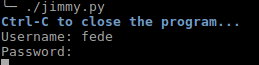
\includegraphics[scale=.8]{img/py.png}
	\caption{Login da terminale - lato client}\label{img:pythonTerminale}
\end{figure}

Tenendo a mente la visione dei sistemi embedded, dalle capacità computazionali ridotte rispetto ad un laptop o ad un PC desktop, si è deciso di utilizzare:
\begin{itemize}
	\item \href{https://github.com/pyserial/pyserial}{pyserial} : per la lettura dei dati dalla seriale;
	\item \href{https://github.com/pyserial/pyserial}{ujson}: per i messaggi JSON;
	\item \href{https://github.com/python/asyncio}{asyncio} : per eseguire le routine in maniera asincrona;
	\item \href{https://github.com/KeepSafe/aiohttp}{aiohttp}: come HTTP client per asyncio.
\end{itemize}
Per poter utilizzare lo script è necessario autenticarsi e ricevere il token JWS al fine di effettuare le richieste HTTP.

\subsubsection{Pyserial}
La libreria \textbf{pyserial} consente la connessione all'Arduino tramite porta seriale e la lettura dei messaggi in maniera continua grazie all'utilizzo di un thread che agisce da produttore di messaggi per l'intero script.

L'elaborazione di questi messaggi viene effettuata da una routine che dopo aver decodificato il messaggio lo instrada al corretto destinatario. Se si deve inviare un messaggio al server, viene composto il messaggio in JSON e viene inviato tramite una richiesta HTTP POST al server.

\subsubsection{Asyncio}
A parte il thread creato per la lettura dei messaggi da Arduino, le altre \textit{routine}, o meglio, \textit{\textbf{coroutine}} sono eseguite all'interno dell'event loop di asyncio. 

Asyncio fornisce una infrastruttura single-threaded per la scrittura di codice concorrente utilizzando coroutine, in particolare è consigliato per \textbf{programmi concorrenti IO-bound}. 

\subsubsection{Aiohttp}
Aiohttp fornisce un supporto per richieste HTTP asincrone tramite l'infrastruttura messa a disposizione da asyncio.

Questo tipo di approccio:
\begin{itemize}
	\item permette di ridurre i consumi di risorse;
	\item aumentare le performance dell'applicazione.
\end{itemize}
Questo risultato si ottiene perché la maggior parte dell'esecuzione dello script è basata sull'invio di dati al server.\\\\
L'obiettivo di rendere completamente asincrono il codice ed eliminare il thread della libreria \textit{pyserial} sarebbe possibile utilizzando delle API per \textit{asyncio} che sono però ancora incomplete ed non affidabili.
\chapter{Testing}

\section{Partita single player}
In questo testing sono state verificate:
\begin{itemize}
	\item la creazione random del numero segreto;
	\item la creazione di nuovi livelli;
	\item la segnalazione del livello giocato sul LED a 12 pin;
	\item la corretta rilevazione della distanza sensore-mano;
	\item le tempistiche di accensione del LED RGB corrette;
	\item la variazione dei suoni emessi dal buzzer se si è dentro/fuori il range del lucchetto;
	\item il dimmeraggio/luce fissa del LED verde se si è dentro/fuori il range del lucchetto;
	\item la visualizzazione del numero segreto premendo il button;
	\item la \textbf{routine di fine gioco}:
	\begin{itemize}
		\item carosello dei LED a 12 pin giallo e rosso;
		\item il dimmeraggio temporizzato del LED verde;
		\item la possibilità di avviare l'\textit{easter egg}.
	\end{itemize}
\end{itemize}

Il testing è stato svolto su sistema operativo GNU/Linux \href{https://manjaro.github.io/}{Manjaro}\footnote{Manjaro è una distribuzione GNU/Linux user-friendly basata sullo sviluppato indipendentemente di Arch Linux. All'interno della comunità Linux, Arch è famoso per essere una distribuzione estremamente veloce, potente e leggera che fornisce l'accesso alla versione più recente del software.}.

\begin{figure}[!ht]
	\centering
	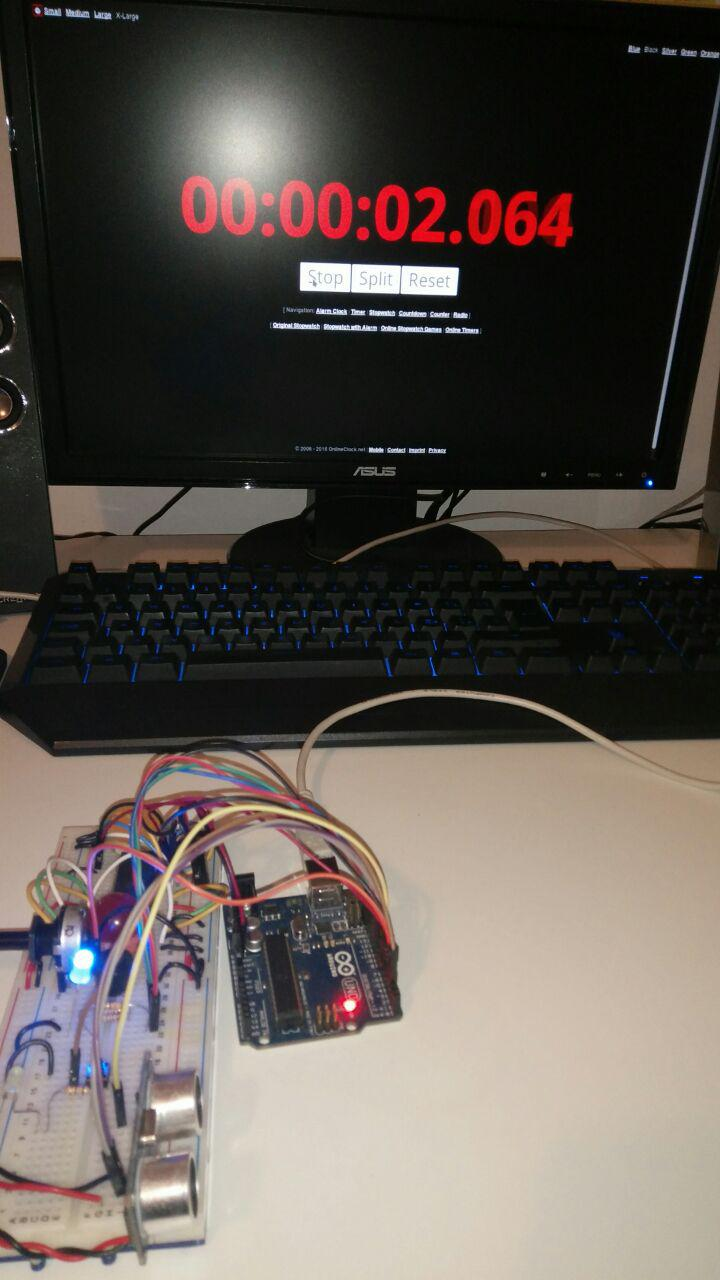
\includegraphics[scale=.25]{img/testing/testing1.jpg}
	\caption{\href{https://youtu.be/X0QOKkfVF4Y}{Testing cronometrato}}
\end{figure}

\clearpage
\section{Web Application - Partita multiplayer}
In questo testing sono state verificate:
\begin{itemize}
	\item la correttezza della comunicazione seriale;
	\item la visualizzazione dello stato dell'avversario.
\end{itemize}

\subsection{Fase di login}
\begin{figure}[!ht]
	\centering
	\begin{subfigure}[b]{0.5\textwidth}
		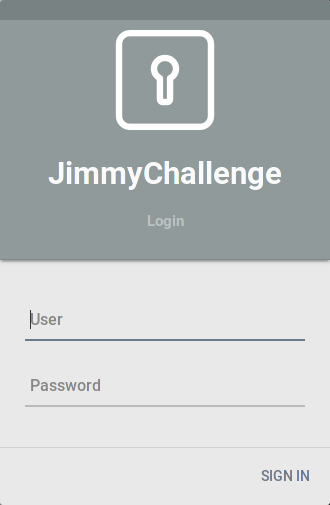
\includegraphics[scale=.4]{img/testing/login.png}
		\caption{Form di login}
	\end{subfigure}
	\begin{subfigure}[b]{0.4\textwidth}
		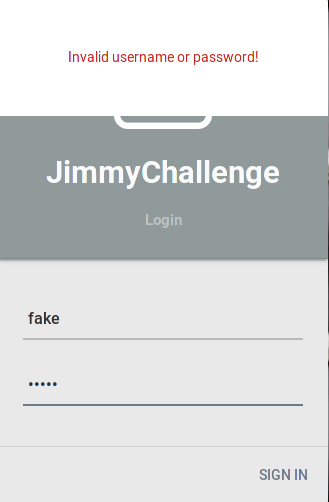
\includegraphics[scale=.4]{img/testing/login_error.png}
		\caption{Errore di login}
	\end{subfigure}
\end{figure}

\clearpage
\subsection{Fase di gioco}
Di seguito sono elencate le fasi di gioco che potrebbero verificarsi.

Per il test da entrambi i giocatori è stato utilizzato il browser Mozilla Firefox e Python 3 su sistema operativo GNU/Linux \href{https://manjaro.github.io/}{Manjaro}.

\begin{figure}[!ht]
	\centering
	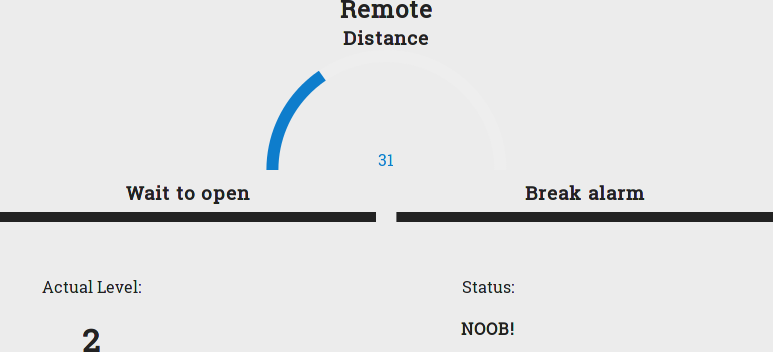
\includegraphics[scale=.4]{img/testing/game1.png}
	\caption{Pistoncino non trovato}
\end{figure}

\begin{figure}[!ht]
	\centering
	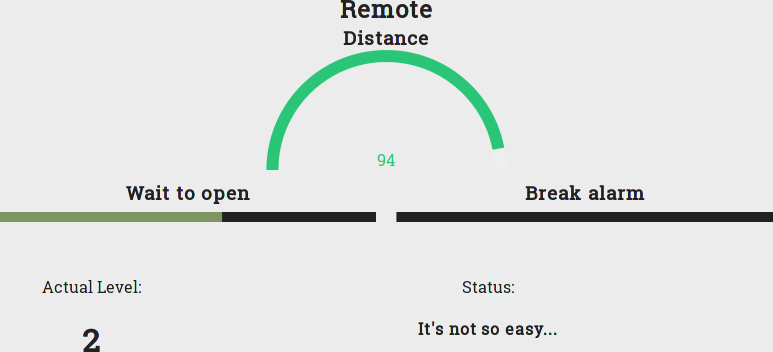
\includegraphics[scale=.4]{img/testing/game2.png}
	\caption{Pistoncino trovato, inizio stato di scasso}
\end{figure}

\begin{figure}[!ht]
	\centering
	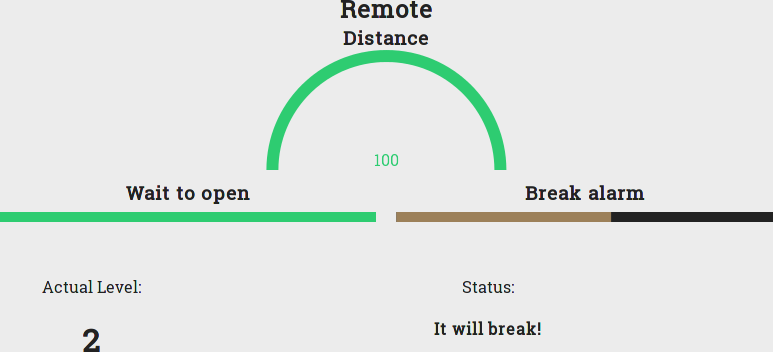
\includegraphics[scale=.4]{img/testing/game3.png}
	\caption{Stato di scasso, rischio rottura}
\end{figure}

\begin{figure}[!ht]
	\centering
	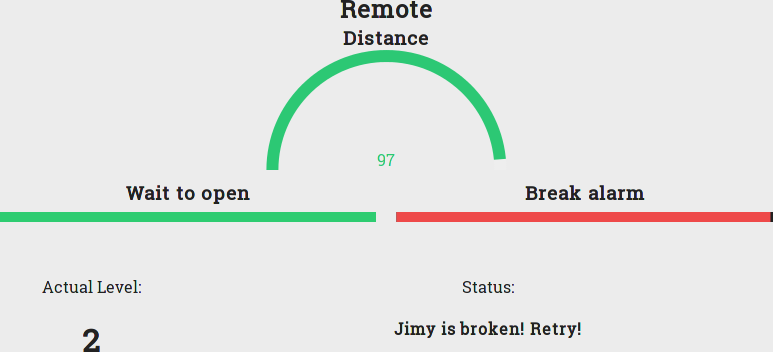
\includegraphics[scale=.4]{img/testing/game4.png}
	\caption{Grimaldello rotto}
\end{figure}

\begin{figure}[!ht]
	\centering
	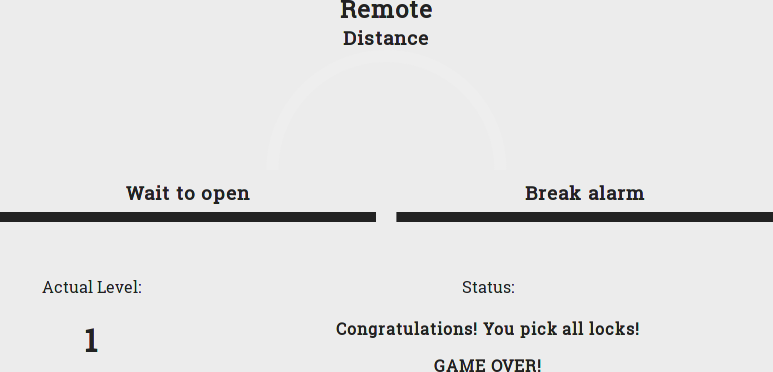
\includegraphics[scale=.4]{img/testing/game5.png}
	\caption{Gioco finito}
\end{figure}


\appendix
\chapter{Elenco dei componenti utilizzati}

\section{Componenti hardware}
\begin{itemize}
	\item Componenti lato client:
	\begin{itemize}
		\item Arduino UNO;
		\item resistori;
		\item sensore di prossimità ad ultrasuoni HC-SR04;
		\item buzzer;
		\item potenziometro;
		\item multiplexer CD4067B;
		\item button;
		\item LED verde;
		\item LED RGB;
		\item LED rosso a 12 pin;
		\item LED giallo a 12 pin;
		\item breadboard;
		\item cavi di collegamento;
	\end{itemize}
\end{itemize}

\begin{itemize}
	\item Componenti lato server:
	\begin{itemize}
		\item Odroid C2;
		\item monitor LCD;
		\item potenziometro;
		\item breadboard;
		\item cavi di collegamento.
	\end{itemize}
\end{itemize}

\section{Componenti software}
\subsection{Librerie Arduino}
\begin{itemize}
	\item \href{http://playground.arduino.cc/Code/NewPing}{NewPing};
	\item \href{https://github.com/bblanchon/ArduinoJson}{ArduinoJson}.
\end{itemize}

\subsubsection{\underline{\href{http://playground.arduino.cc/Code/NewPing}{NewPing}}}\label{sec:newping}
\textbf{Caratteristiche}
\begin{itemize}
	\item Funziona con diversi modelli di sensori ad ultrasuoni: SR04, SRF05, SRF06, DYP-ME007 e Parallax Ping™;
	\item Non ha un \textbf{lag} di un secondo se non si riceve un ping di eco
	\item Ping coerente e affidabile fino a 30 volte al secondo.
	\item Timer interrupt method per sketch event-driven
	\item Metodo di filtro digitale Built-in \texttt{ping\_median()} per facilitare la correzione degli errori.
	\item Utilizzo dei registri delle porte durante l'accesso ai pin per avere un'esecuzione più veloce e dimensioni del codice ridotte.
	\item Consente l'impostazione di una massima distanza di lettura del ping "in chiaro".
	\item Facilita l'utilizzo di più sensori.
	\item Calcolo distanza preciso, in centimetri, pollici e uS.
	\item Non fa uso di \texttt{pulseIn}, in quanto lento e con alcuni modelli di sensore a ultrasuoni restituisce risultati errati.
	\item Attualmente in sviluppo, con caratteristiche che vengono aggiunte e bug/issues affrontati.
\end{itemize}

\subsubsection{\underline{\href{https://github.com/bblanchon/ArduinoJson}{ArduinoJson}}}\label{sec:arduinojason}
\textbf{Caratteristiche}
\begin{itemize}
	\item codifica/decodifica JSON;
	\item API di facile utilizzo;
	\item allocazione di memoria fissa (senza malloc);
	\item nessuna \textit{data duplication} (evitando la copia);
	\item portatile (scritto in C++98);
	\item non ha dipendenze esterne;
	\item libreria leggera;
	\item MIT License.
\end{itemize}

\subsection{IDE utilizzati}
\begin{itemize}
	\item \href{https://atom.io/}{Atom} con \href{ http://platformio.org/}{PlatformIO};
	\item \href{https://www.arduino.cc/en/Main/Software}{Arduino IDE} (per alcuni test sulla comunicazione seriale).
\end{itemize}

\subsection{Linguaggi di sviluppo}
\begin{itemize}
	\item Wiring/C++;
	\item Python;
	\item JSON;
	\item HTML;
	\item ....
\end{itemize}

\subsection{Altro}
\begin{itemize}
	\item \href{http://fritzing.org}{Fritzing} per riportare gli schemi di collegamento.
\end{itemize}
\chapter{Schema di collegamento}
\section{Sketch Arduino - lato client}
\begin{figure}[!ht]
	\centering
	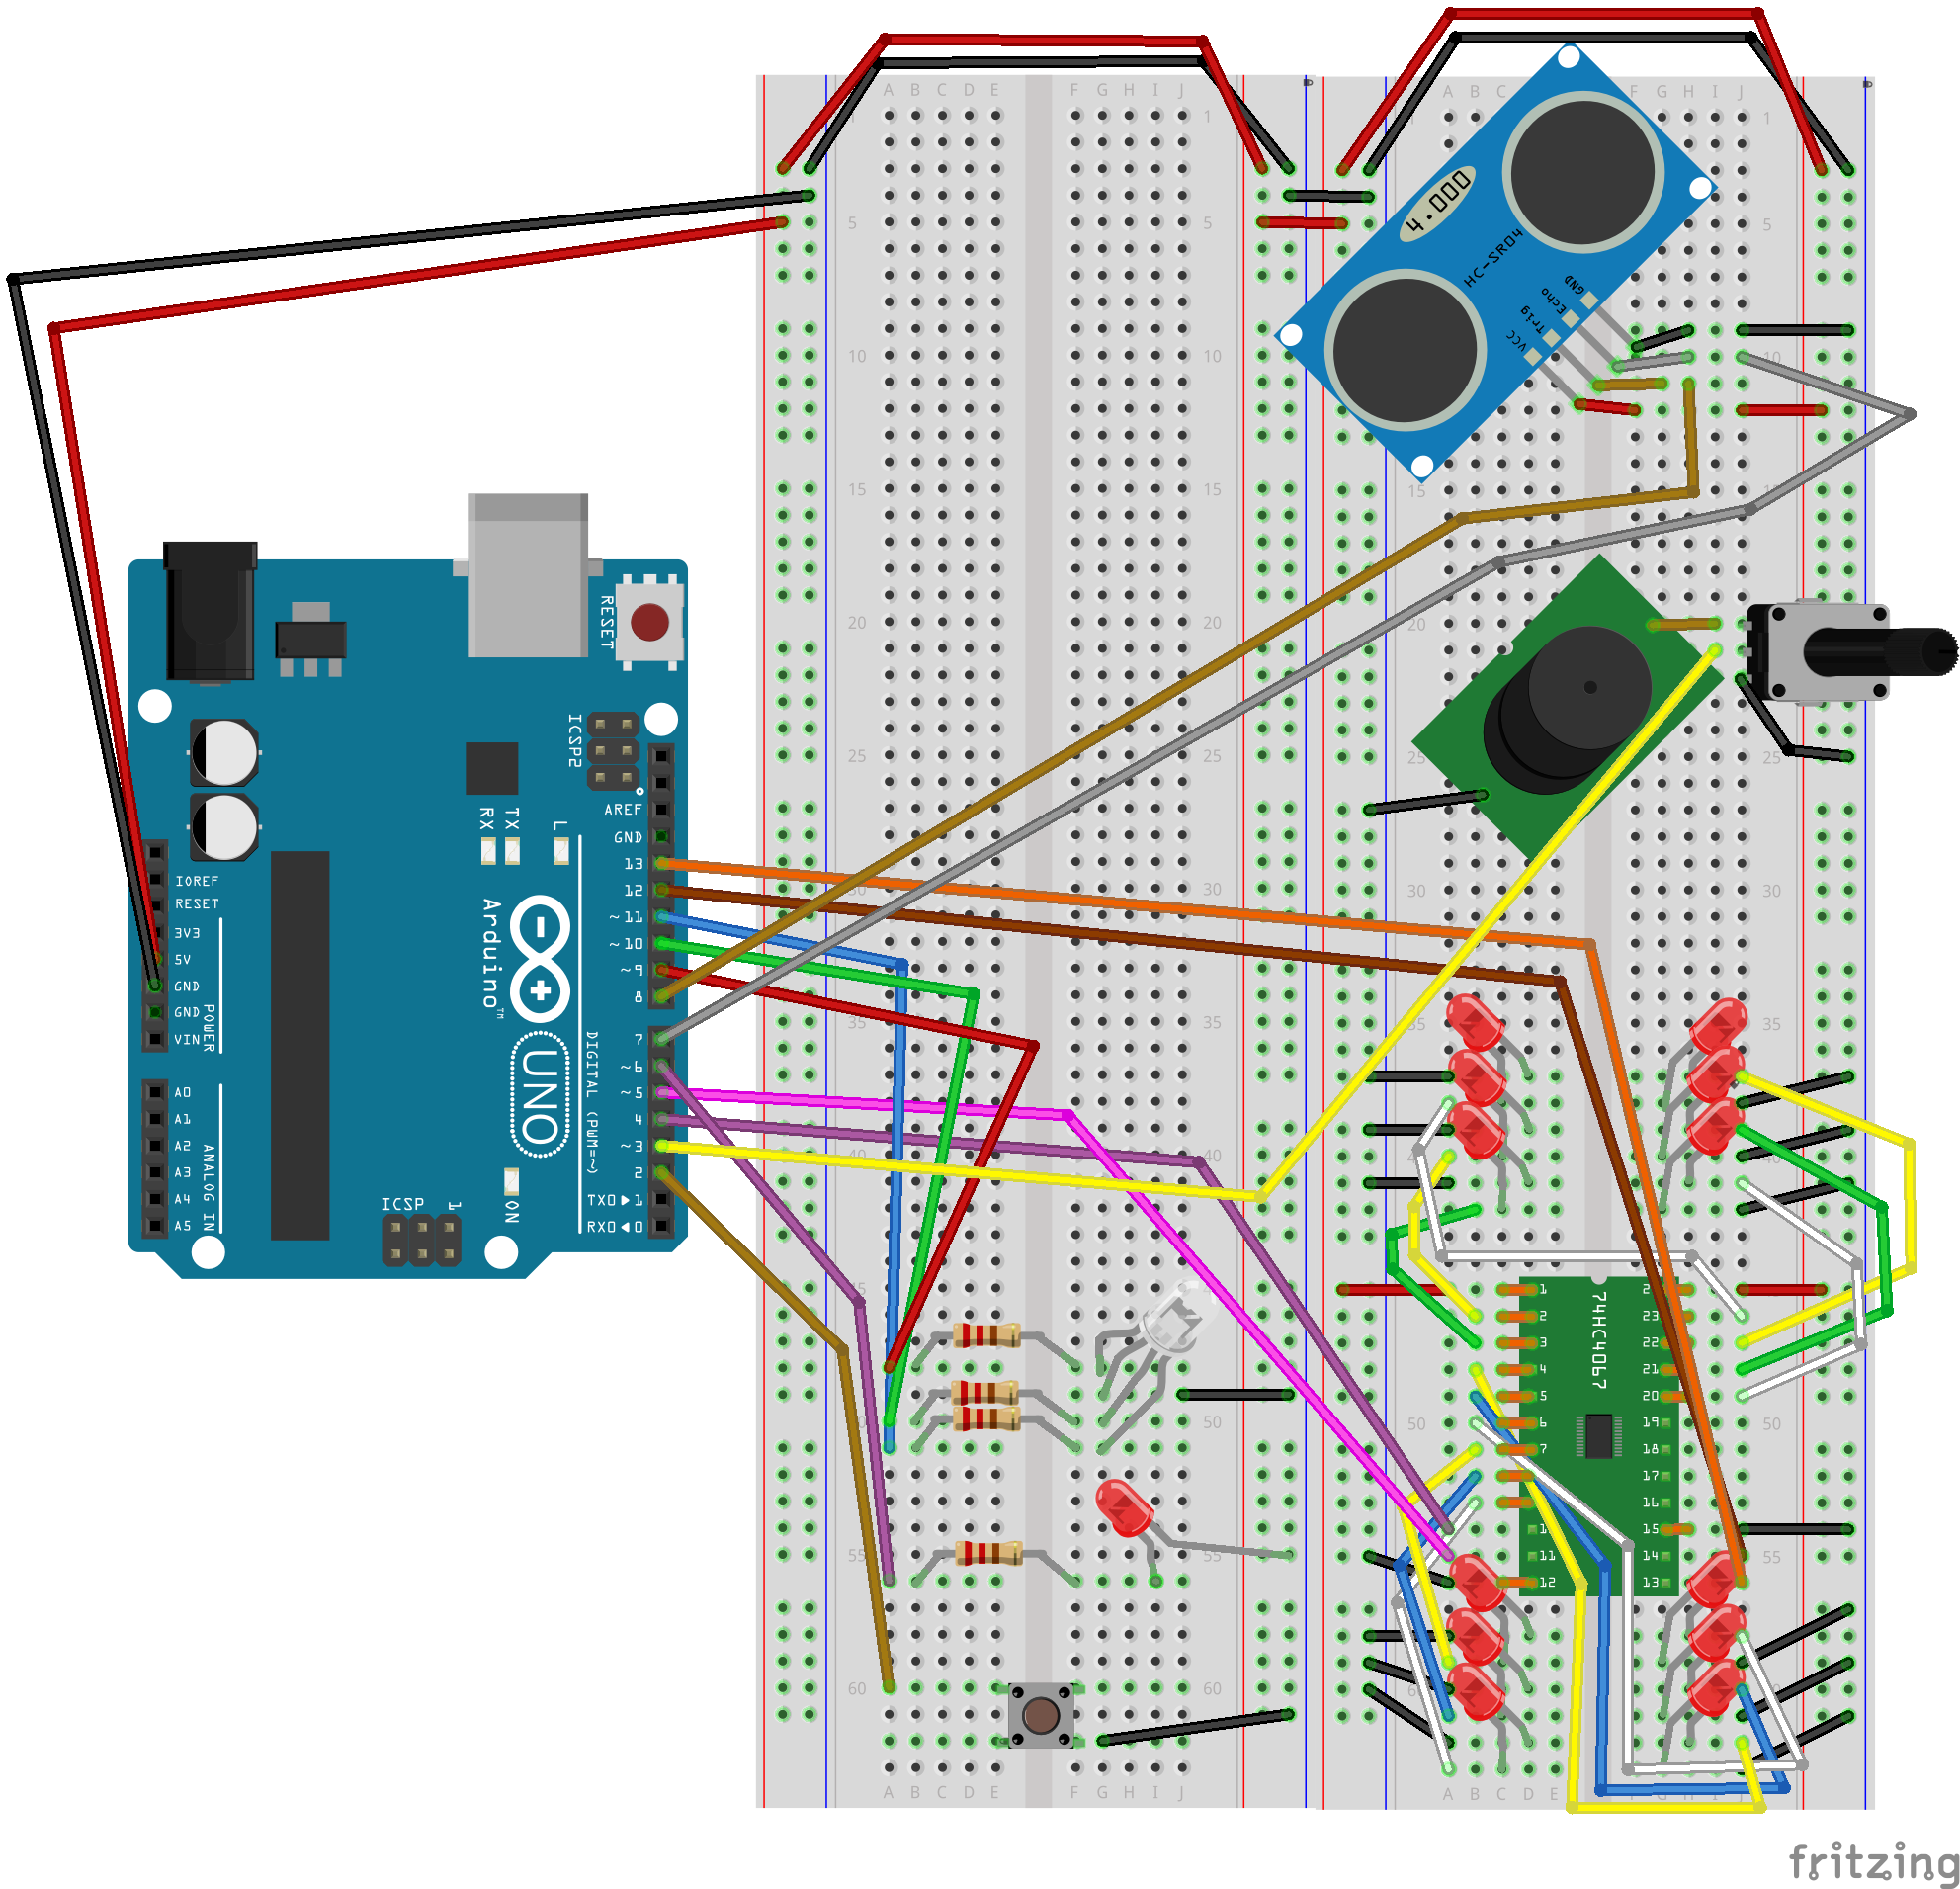
\includegraphics[scale=.60]{img/SketchClient.png}
	\caption{Sketch Arduino - fritzing}
\end{figure}

\begin{figure}[!ht]
	\centering
	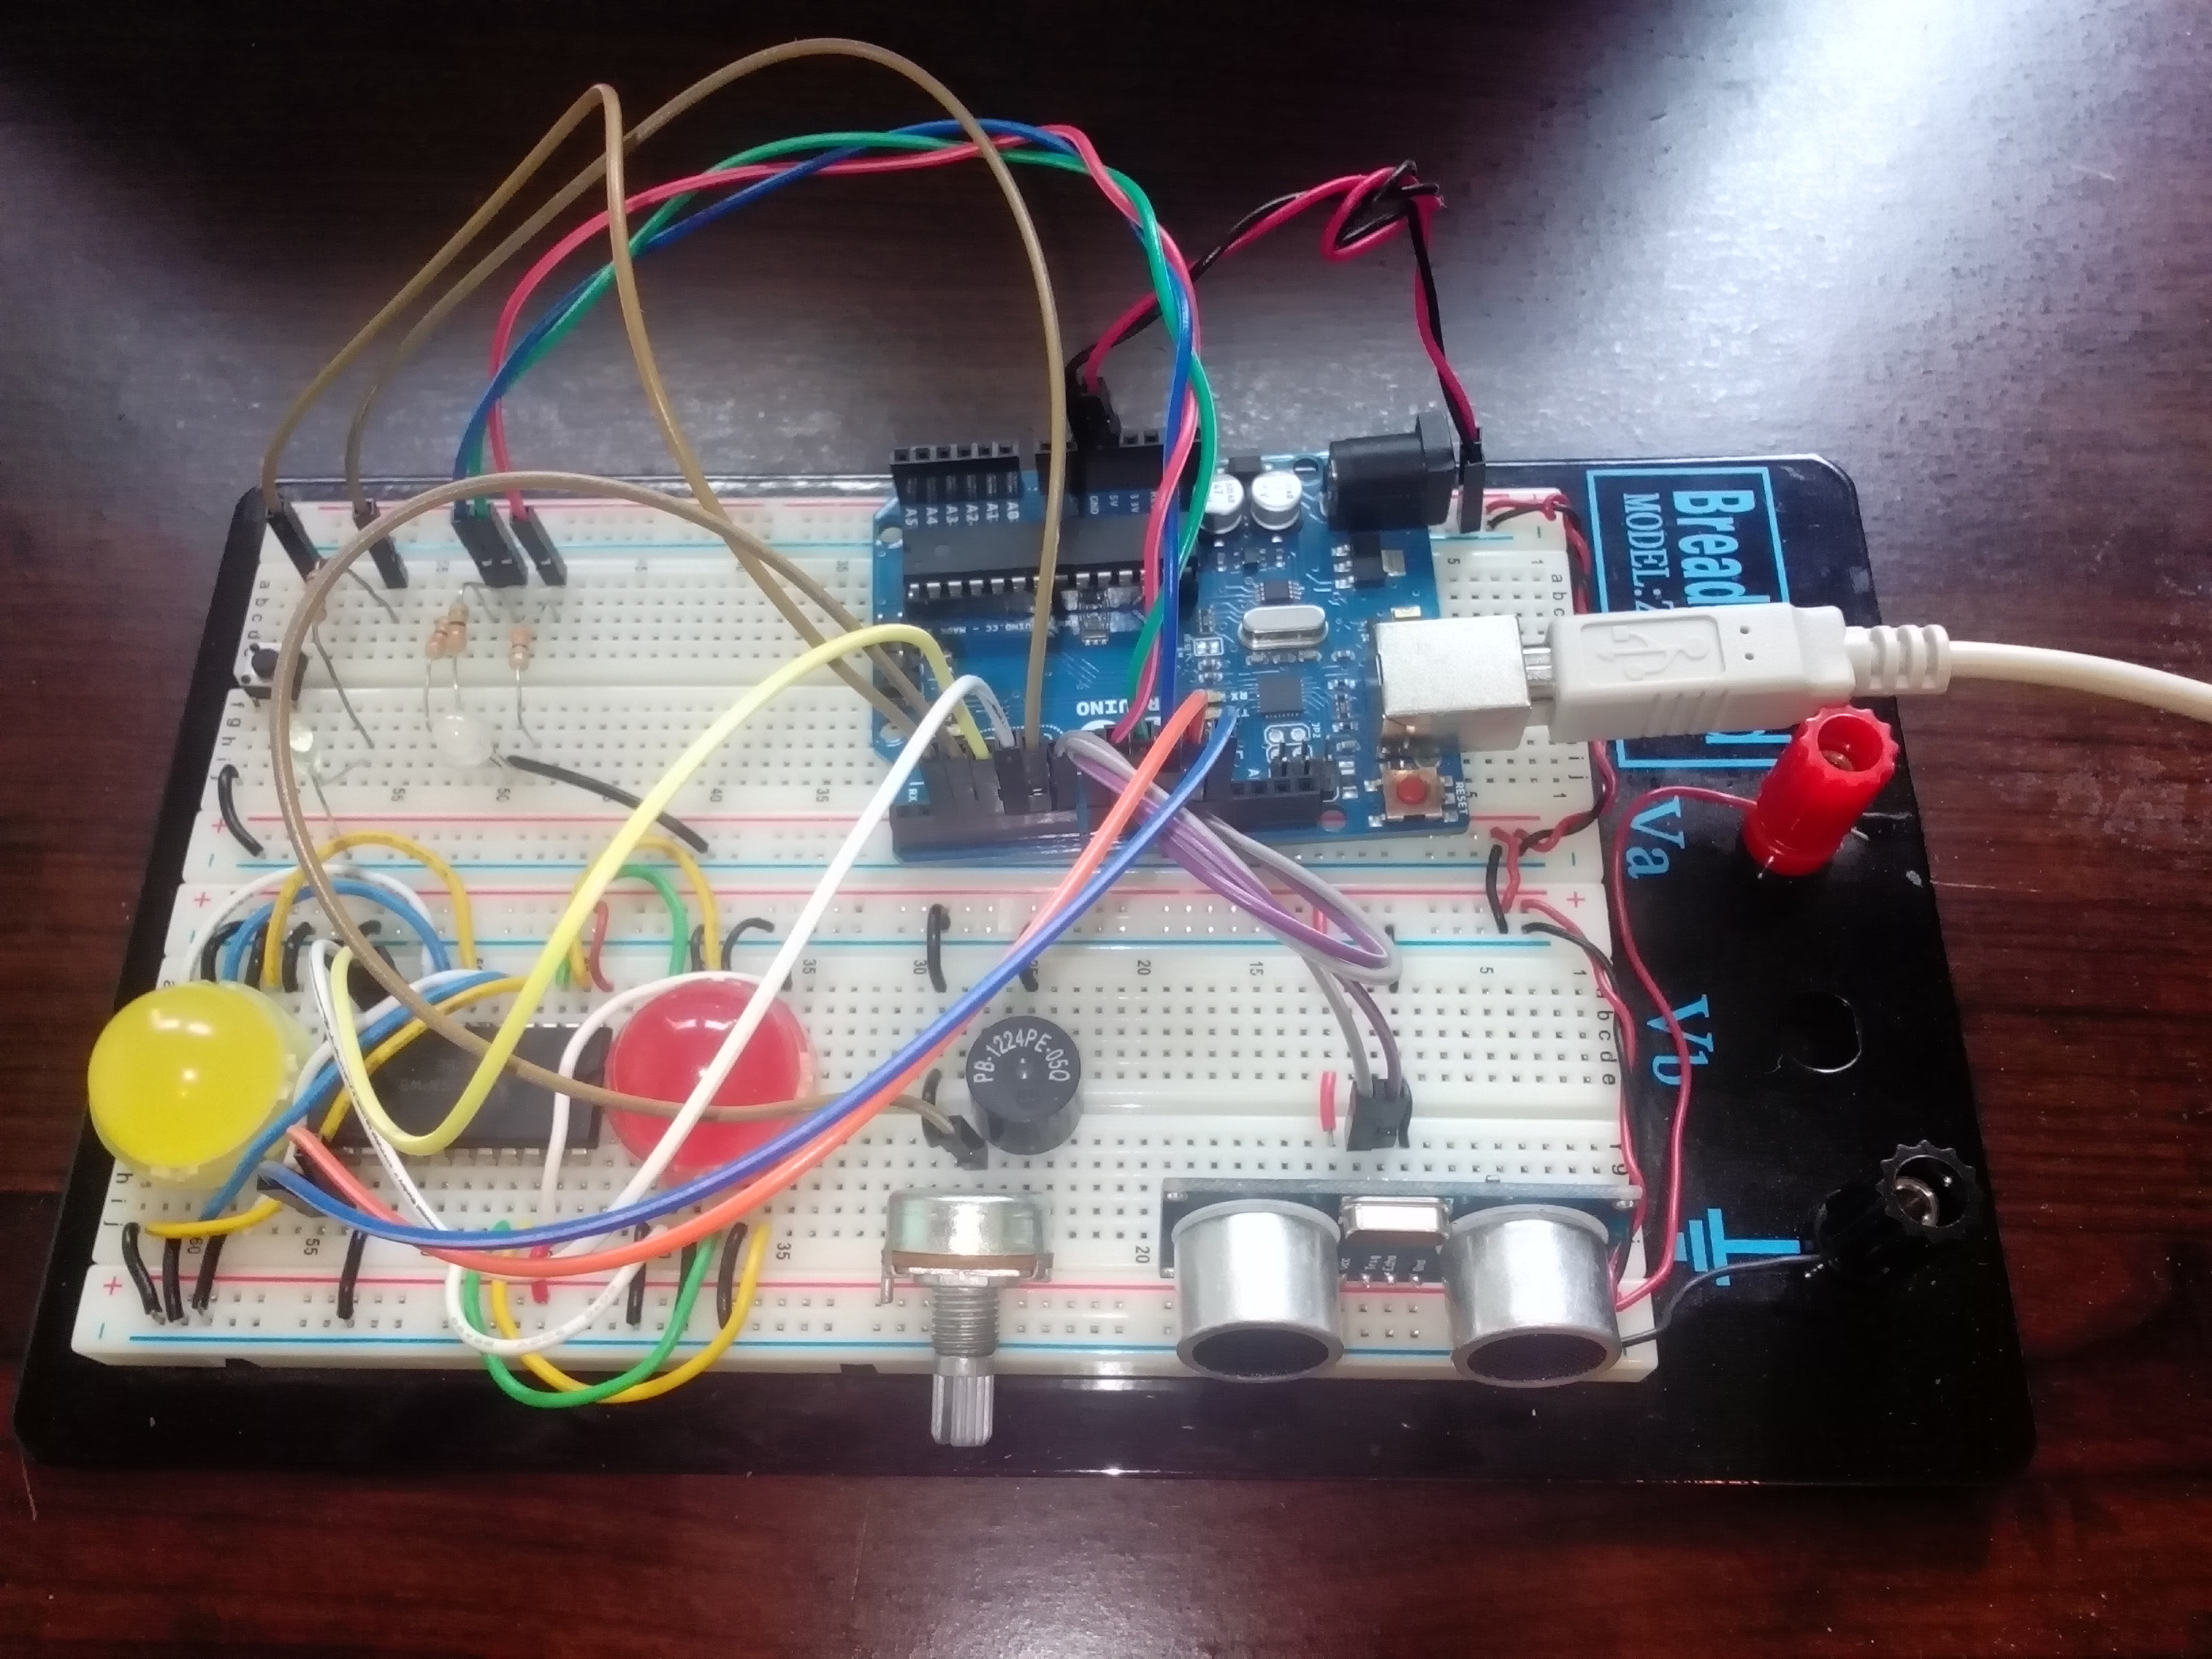
\includegraphics[scale=.08]{img/real1.jpg}
	\caption{Sketch Arduino - realizzazione reale}
	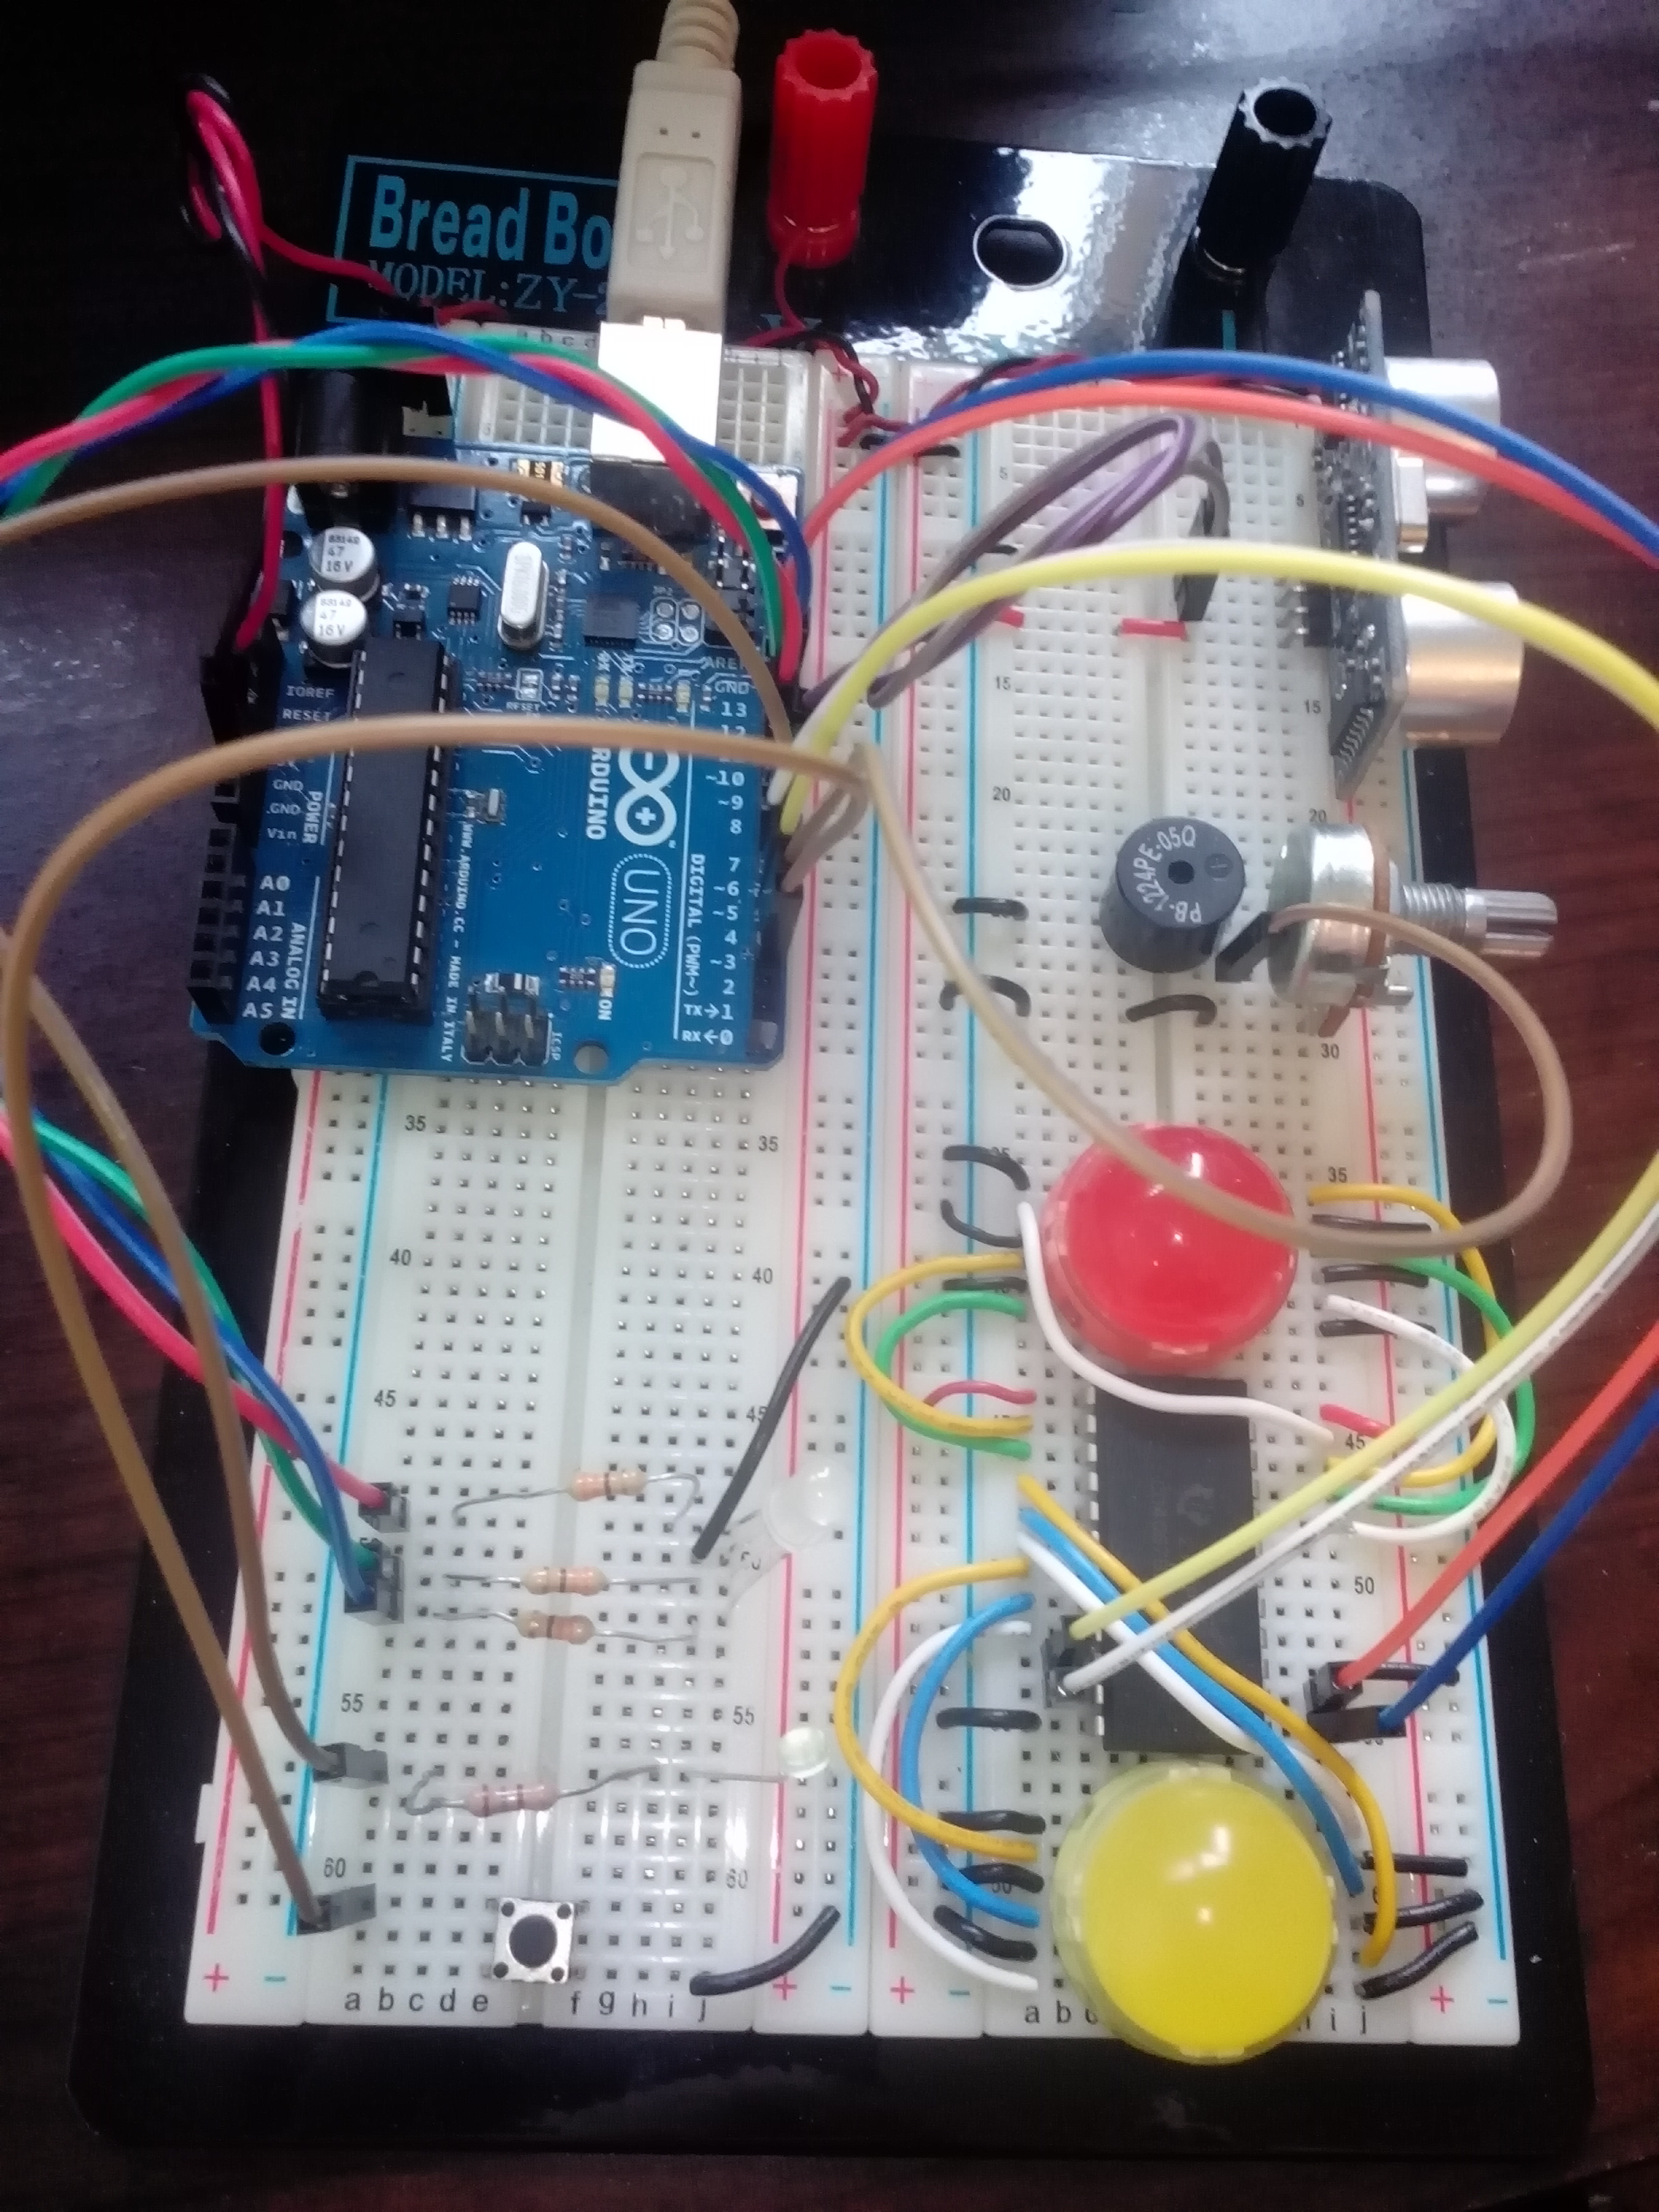
\includegraphics[scale=.08]{img/real2.jpg}
	\caption{Sketch Arduino - realizzazione reale}
\end{figure}

\clearpage
\section{Sketch Odroid - lato server}
\begin{figure}[!ht]
	\centering
	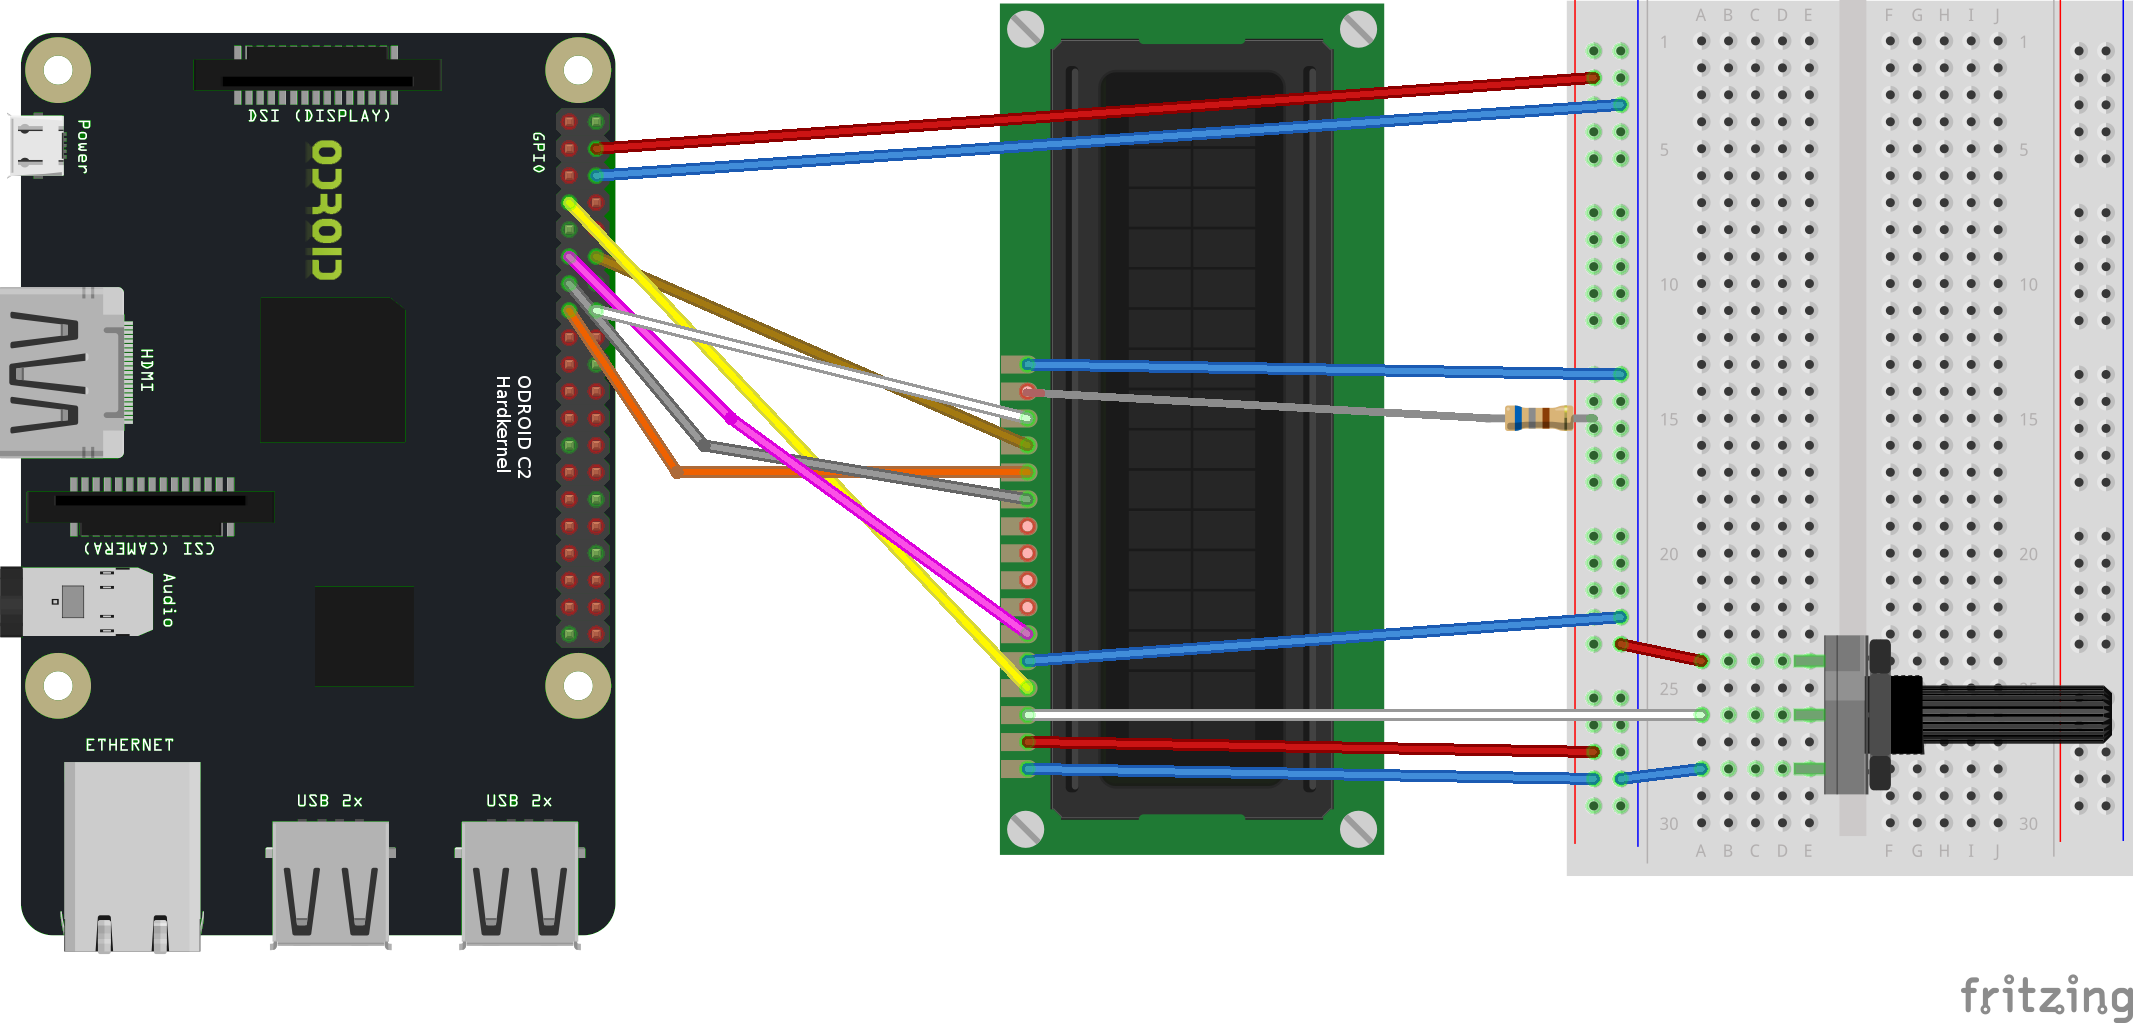
\includegraphics[scale=.2]{img/SketchServer.png}
	\caption{Sketch Arduino - fritzing}
\end{figure}

\begin{figure}[!ht]
	\centering
	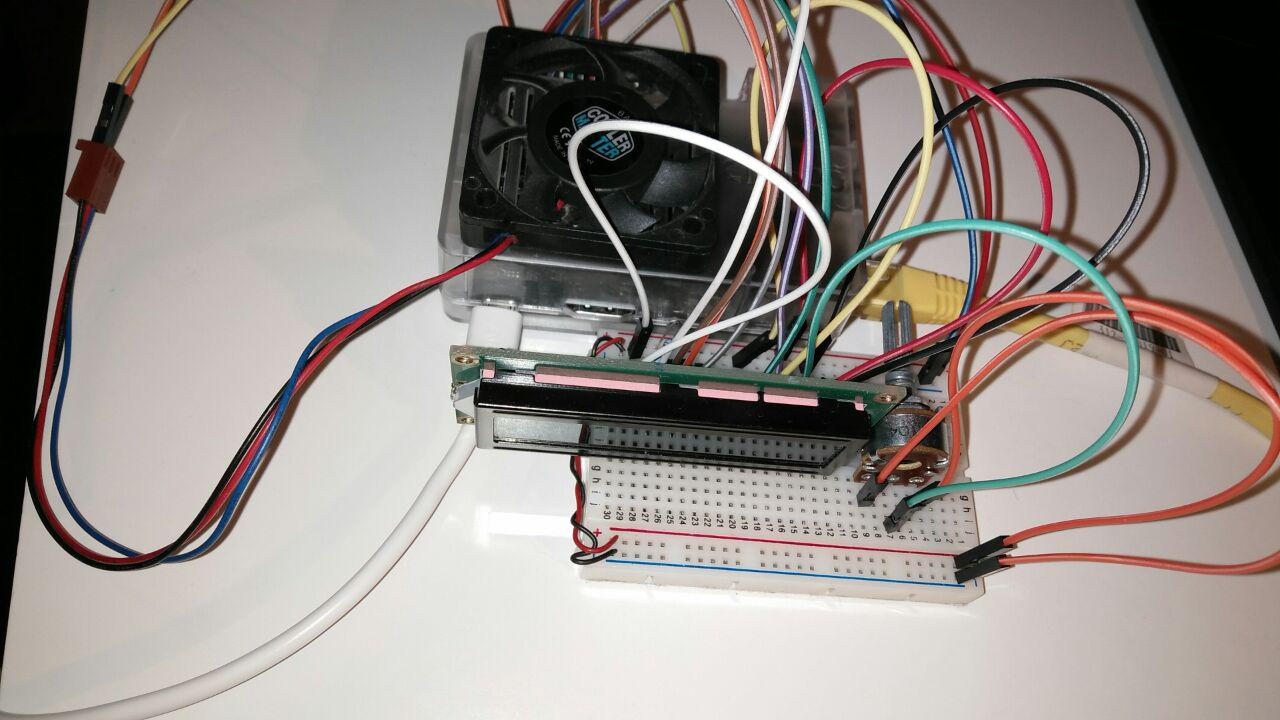
\includegraphics[scale=.3]{img/real3.jpg}
	\caption{Sketch Odroid - realizzazione reale}
	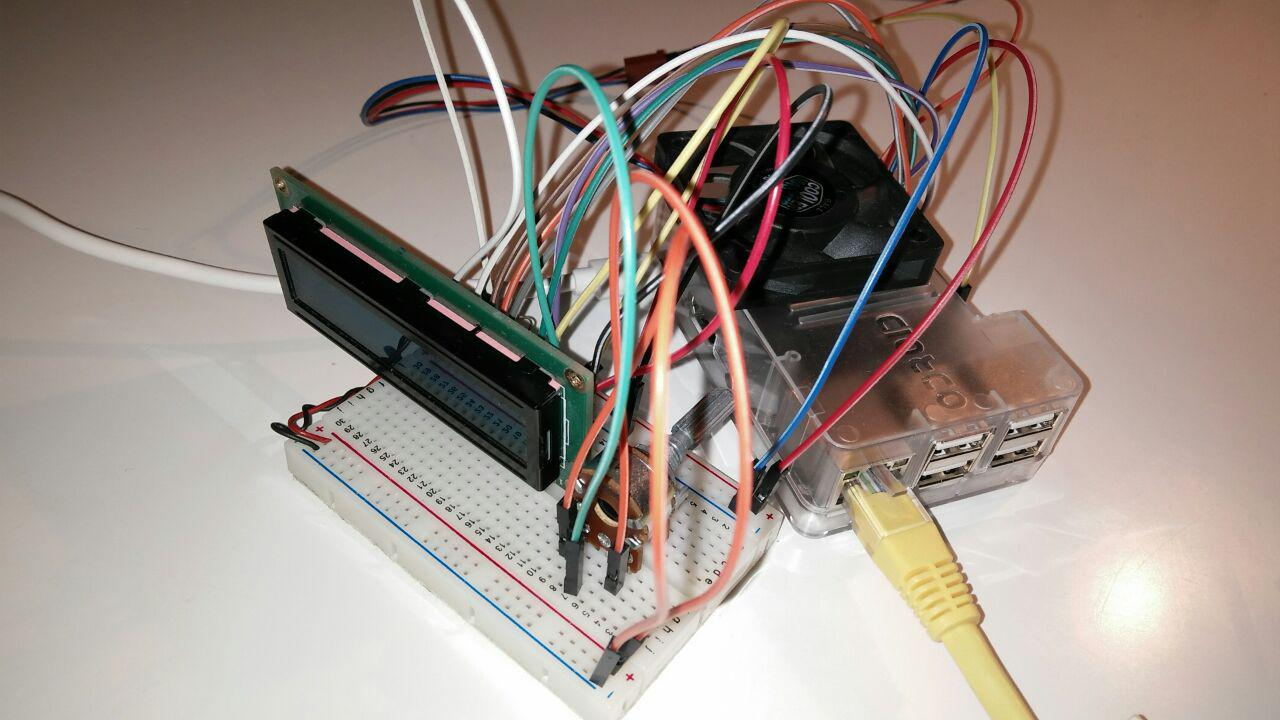
\includegraphics[scale=.3]{img/real4.jpg}
	\caption{Sketch Odroid - realizzazione reale}
\end{figure}
\end{document}               % End of document.
